\documentclass[12pt,a4paper]{report}

% -----------------------------
% Packages (deduped and ordered)
% -----------------------------
\usepackage[top=3cm,right=3cm,bottom=3cm,left=2.5cm]{geometry}
\usepackage{amsmath}
\usepackage{graphicx}
\usepackage{subfigure}
\usepackage{float}
\usepackage{caption}
\usepackage{indentfirst}
\usepackage{listings}
\usepackage{xcolor}
\usepackage{caption}   % for \captionof
\usepackage{booktabs}  % (optional) for \toprule etc.
\usepackage{needspace} % to keep heading + table together nicely
\usepackage{tikz}
\usetikzlibrary{arrows.meta, positioning, fit, shapes.geometric, shapes.misc}
\tikzstyle{startstop} = [rectangle, rounded corners, minimum width=3cm, minimum height=1cm,text centered, draw=black, fill=red!30]
\tikzstyle{process} = [rectangle, minimum width=3.5cm, minimum height=1cm, text centered, draw=black, fill=blue!20]
\tikzstyle{arrow} = [thick,->,>=stealth]
\usepackage{fancyhdr}
\usepackage[hang,flushmargin]{footmisc}
\usepackage{booktabs}
\usepackage{amsmath}
\usepackage{amssymb}
\usepackage{amsfonts}

% Load hyperref LAST
\usepackage[hidelinks]{hyperref}

% -----------------------------
% Headers / Footers
% -----------------------------
\pagestyle{fancy}
\fancyhf{}
\fancyhead[R]{\thepage}
\renewcommand{\headrulewidth}{0pt}

\fancypagestyle{plain}{
  \fancyhf{}
  \fancyhead[R]{\thepage}
  \renewcommand{\headrulewidth}{0pt}
}

% -----------------------------
% Numbering formats (kept, but no trailing dashes)
% -----------------------------
\renewcommand{\thesection}{\thechapter-\arabic{section}}
\renewcommand{\thesubsection}{\thechapter-\arabic{section}-\arabic{subsection}}
\renewcommand{\thesubsubsection}{\thechapter-\arabic{section}-\arabic{subsection}-\arabic{subsubsection}}

\renewcommand{\thetable}{(\thechapter-\arabic{table})}
\renewcommand{\thefigure}{(\thechapter-\arabic{figure})}
\captionsetup{font=small,labelsep=space}

% -----------------------------
% Document
% -----------------------------
\begin{document}

% -----------------------------
% Front Matter (Unnumbered)
% -----------------------------
\pagenumbering{roman}

\chapter*{Abstract}
% Write your abstract here.

\chapter*{Acknowledgements}
% Write your acknowledgements here.

\tableofcontents
\listoffigures
\listoftables

% -----------------------------
% Main Content (Numbered Chapters)
% -----------------------------
\pagenumbering{arabic}

\chapter{Introduction}

\section{Objectives and Scope}

The primary objective of this research is to investigate whether reinforcement learning (RL) agents, enhanced with sentiment information from large language models (LLMs), can improve trading performance in the context of the Dow Jones Industrial Average (Dow30). RL methods have been increasingly applied in algorithmic trading and portfolio management \cite{pricope2021deep}, making them a suitable foundation for this study. To achieve this, the study pursues the following specific objectives:

\begin{itemize}
    \item Develop and evaluate reinforcement learning agents for Dow30 trading.
    \item Integrate sentiment features from FinBERT \cite{araci2019finbert}, FinGPT \cite{yang2023fingpt}, and Google News with market and technical data.
    \item Compare the performance of the proposed models against traditional models \cite{markowitz1952portfolio}, basic benchmark strategies, and findings from recent academic research.
    \item Examine the influence of state and action space design, reward shaping, and hyperparameter choices on model effectiveness.
    \item Assess the impact of advanced architectures such as LSTM \cite{hochreiter1997lstm}, Transformers \cite{vaswani2017attention}, and Proximal Policy Optimization (PPO) \cite{schulman2017proximal} on trading performance.
\end{itemize}

The scope of this study is defined as follows:

\begin{itemize}
    \item The analysis is restricted to Dow30 index constituents and does not extend to other asset classes or global markets.
    \item Market data is limited to OHLCV data and sentiment signals obtained from FinBERT \cite{araci2019finbert}, FinGPT \cite{yang2023fingpt}, and Google News. Alternative data sources, such as social media or order book data, are excluded.
    \item The focus is on daily trading horizons, with ultra-high-frequency trading outside the scope of this research.
    \item The models are implemented and evaluated under research-oriented conditions and are not intended as production-ready trading systems.
    \item Evaluation is based on commonly used performance and risk metrics (e.g., Sharpe ratio, drawdown, volatility), while long-term portfolio optimization and capital allocation strategies are not addressed.
\end{itemize}


\section{Applications and Practical Relevance}

The development of reinforcement learning (RL) agents enhanced with large language models (LLMs) carries significant practical potential in the domain of algorithmic trading and portfolio management. By combining market-structured data with unstructured sentiment information, such systems can support more adaptive and context-aware decision-making, thereby improving risk-adjusted performance. The proposed framework is not limited to theoretical experimentation but is directly applicable to automated trading pipelines, investment decision support systems, and financial risk monitoring platforms.

Although direct trading in international stock markets is currently not feasible from Iran due to regulatory and geopolitical constraints, practical deployment remains possible through the use of intermediary brokers and online trading platforms such as RoboForex and similar providers. These intermediaries grant access to global equity indices, foreign exchange, and other asset classes, enabling the integration of RL-based agents into real-world trading scenarios. Thus, while the models presented in this study are research-oriented, they can be adapted and connected to brokerage APIs for semi-automated or fully automated execution in practice.

The timing of this research is particularly relevant. With the rapid progress of both reinforcement learning and LLM technologies, financial markets are entering a new era of AI-driven decision-making. The ability of RL to optimize sequential strategies and of LLMs to interpret vast streams of textual and sentiment information provides a synergistic advantage for investors. In an era defined by volatility, globalization, and the increasing importance of information-driven trading, systems that integrate RL and LLMs can provide substantial financial benefits, ranging from enhanced returns to more robust risk management.



\section{Research Questions and Hypotheses}

This study is guided by the following research questions and their corresponding hypotheses:

\subsection*{Performance of RL vs. Traditional and Contemporary Approaches}
\begin{itemize}
    \item \textbf{RQ1:} Can reinforcement learning agents outperform traditional models, basic benchmark strategies, and approaches reported in recent academic research when applied to Dow30 and other market trading tasks? \\
    \textbf{H1:} Reinforcement learning agents are expected to achieve higher risk-adjusted returns compared to traditional models and baseline strategies in Dow30 and other market trading tasks, but may not consistently outperform the most recent state-of-the-art approaches documented in current research.

    \item \textbf{RQ2:} How does the proposed model compare against traditional baselines, benchmark strategies, and contemporary research methods in terms of risk-adjusted performance, profitability, and robustness? \\
    \textbf{H2:} The proposed model is hypothesized to outperform traditional baselines and benchmark strategies in terms of profitability, stability, and robustness across different market conditions.
\end{itemize}

\subsection*{Impact of Sentiment and Market Data}
\begin{itemize}
    \item \textbf{RQ3:} Does incorporating sentiment features obtained from FinBERT, FinGPT, and Google News improve trading performance compared to price-based models alone? \\
    \textbf{H3:} Incorporating sentiment features from FinBERT \cite{araci2019finbert}, FinGPT \cite{yang2023fingpt}, and Google News is expected to improve trading performance relative to models using only price-based data.
    
    \item \textbf{RQ4:} Do sentiment features and traditional technical indicators exhibit significant correlations, and how does this relationship affect model performance? \\
    \textbf{H4:} Sentiment features and technical indicators are hypothesized to exhibit significant but non-trivial correlations, and jointly incorporating them will enhance model performance.
    
    \item \textbf{RQ5:} How does reward shaping and the design of action and state spaces influence the performance of RL-based trading models? \\
    \textbf{H5:} Reward shaping and careful design of action and state spaces are expected to positively influence the performance of reinforcement learning-based trading agents.
\end{itemize}

\subsection*{Model Architectures and Hyperparameters}
\begin{itemize}
    \item \textbf{RQ6:} Does combining LSTM with reinforcement learning algorithms such as Recurrent PPO (RPPO) consistently improve performance? \\
    \textbf{H6:} Combining LSTM architectures \cite{hochreiter1997lstm} with reinforcement learning algorithms such as Recurrent PPO is hypothesized to enhance model performance by improving sequential pattern recognition.
    
    \item \textbf{RQ7:} Can encoding the state space with advanced architectures such as Transformers or LSTMs lead to better results than traditional encodings? \\
    \textbf{H7:} State encoding with advanced architectures such as Transformers \cite{vaswani2017attention} or LSTMs \cite{hochreiter1997lstm} is expected to outperform simpler encodings in capturing market dependencies.
    
    \item \textbf{RQ8:} Between FinBERT, FinGPT, and hybrid combinations of the two, which provides the most effective sentiment representation for financial trading? \\
    \textbf{H8:} Hybrid combinations of FinBERT and FinGPT are hypothesized to provide more effective sentiment representations for financial trading than either model individually.
    
    \item \textbf{RQ9:} To what extent do algorithmic hyperparameters affect the performance and stability of RL-based trading strategies? \\
    \textbf{H9:} Algorithmic hyperparameters are expected to have a significant impact on the performance and stability of reinforcement learning-based trading models.
\end{itemize}




\section{Structure of Report}

The report is organized into eight chapters. \textbf{Chapter 2} introduces the theoretical foundations of this work. It begins with the fundamentals of reinforcement learning, including its core principles, the exploration--exploitation trade-off, learning paradigms, and distinctions between different approaches. It then reviews major reinforcement learning algorithms such as Q-learning, policy gradient methods, actor--critic frameworks, and advanced techniques like Proximal Policy Optimization (PPO) and Recurrent PPO. In addition, the chapter outlines the fundamentals of large language models (LLMs), covering the transformer architecture, word embeddings, training strategies, and their application to sentiment analysis in finance. It also discusses the structure of market data and financial indicators, as well as portfolio management and trading constraints, including transaction costs, liquidity considerations, and risk measures.  

\textbf{Chapter 3} provides a review of the relevant literature. It surveys research on the application of LLMs in financial natural language processing, available RL libraries and their applications in finance, the use of deep reinforcement learning for financial decision-making, and hybrid approaches that integrate NLP with RL in trading.  

\textbf{Chapter 4} presents the research methodology and overall system design. It formally defines the problem and describes the architecture of the proposed framework. \textbf{Chapter 5} details the implementation process, including the tools and frameworks employed, reproducibility considerations, and the computational resources required.  

\textbf{Chapter 6} outlines the experimental setup and presents the empirical results obtained from evaluating the proposed system. \textbf{Chapter 7} provides a discussion and critical analysis of the findings, emphasizing both contributions and limitations. Finally, \textbf{Chapter 8} concludes the study by summarizing the key insights, reflecting on the implications for financial AI research, and proposing potential directions for future work.  



\chapter{Theoretical Concepts}

\section{Introduction}

This chapter provides the theoretical foundations necessary for understanding the development of a reinforcement learning (RL) agent in the context of financial markets, with an emphasis on the integration of large language models (LLMs). The discussion begins with the basic principles of RL, including its core components, the balance between exploration and exploitation, and distinctions such as on-policy vs. off-policy learning and model-free vs. model-based approaches. Building on this foundation, we then introduce key RL algorithms—ranging from Q-learning and policy gradient methods to actor-critic frameworks and advanced variants such as Proximal Policy Optimization (PPO) and its recurrent extension.  

In addition to RL, the chapter reviews the fundamentals of LLMs, covering the transformer architecture, embedding techniques, and different training paradigms. The role of sentiment analysis in finance is highlighted to illustrate how textual data can complement numerical market indicators. Finally, we examine the structure and challenges of financial market data, portfolio management considerations, and practical constraints such as transaction costs, risk measures, and evaluation metrics. Collectively, these concepts form the theoretical basis for the design and evaluation of the proposed RL-based trading agent enhanced with LLM-driven insights.

\section{RL basics}

\subsection{Core Components}

Reinforcement Learning (RL) is a computational approach to sequential decision-making in which an agent learns to select actions by interacting with an environment. The primary objective is to maximize the cumulative reward signal over time. The fundamental components of an RL framework are illustrated in Figure~\ref{fig:rl_framework}.

\begin{figure}[htbp]
  \centering
  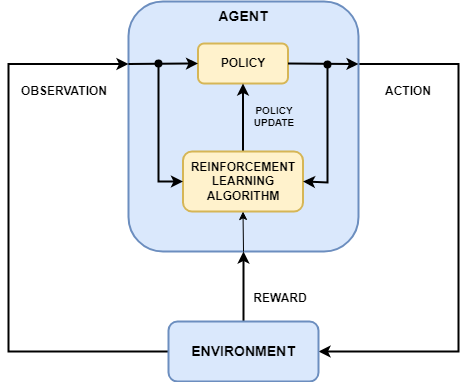
\includegraphics[width=0.75\textwidth]{photos/reinforcement_learning_diagram.png}
  \caption{General framework of Reinforcement Learning~\cite{mathworksRLdiag2025}.}
  \label{fig:rl_framework}
\end{figure}

\begin{itemize}
    \item \textbf{Agent:} The learner or decision maker. In algorithmic trading, the agent corresponds to the trading strategy that chooses between buy, sell, or hold actions.
    
    \item \textbf{Environment:} The external system with which the agent interacts. In financial applications, this typically represents the market, including price dynamics, order book information, and sentiment data.
    
    \item \textbf{State ($s_t$):} A representation of the environment at time $t$. In trading contexts, states may include technical indicators (e.g., moving averages, RSI), sentiment scores derived from news sources, and historical OHLCV\footnote{Open, High, Low, Close, Volume} data.
    
    \item \textbf{Action ($a_t$):} The set of decisions available to the agent at time $t$. In trading, this often corresponds to $\{ \text{buy, sell, hold} \}$, but can also extend to portfolio rebalancing or continuous position sizing.
    
    \item \textbf{Reward ($r_t$):} A scalar feedback signal that quantifies the immediate gain or loss resulting from taking action $a_t$ in state $s_t$. In finance, this is commonly defined as profit and loss (PnL), risk-adjusted returns, or a custom function incorporating risk management objectives.
    
    \item \textbf{Policy ($\pi$):} The agent’s strategy for mapping states to actions. Policies may be deterministic ($a = \pi(s)$) or stochastic ($a \sim \pi(\cdot|s)$).
    
    \item \textbf{Value Function:} An estimate of the expected cumulative reward when starting from a given state (or state-action pair). It provides a measure of the long-term desirability of states beyond immediate rewards.
    
    \item \textbf{Model of the Environment:} An optional component that predicts state transitions given actions. Model-free approaches, such as Proximal Policy Optimization (PPO), do not attempt to explicitly model the environment, whereas model-based methods incorporate such predictive models.
\end{itemize}

These components form the foundation of RL algorithms. In financial trading, careful design of the state space, action set, and reward function is critical, as poor definitions can lead to unstable learning dynamics or unprofitable trading strategies~\cite{sutton2018reinforcement}.

\subsection{Exploration vs. Exploitation}

A central challenge in Reinforcement Learning (RL) is the trade-off between \textit{exploration} and \textit{exploitation}. 

\begin{itemize}
    \item \textbf{Exploration:} The process of selecting less certain actions to acquire new knowledge and potentially discover strategies that yield higher long-term returns. In trading, exploration may involve testing novel indicators or market signals, even if their immediate profitability is unclear.
    
    \item \textbf{Exploitation:} The process of leveraging current knowledge to maximize expected rewards by consistently choosing actions that are estimated to perform best. In financial applications, this corresponds to executing trades that have historically demonstrated strong returns.
\end{itemize}

\begin{figure}[htbp]
  \centering
  
\includegraphics[width=0.75\textwidth]{photos/exp_vs_exp.jpg}
  \caption{Illustration of the exploration–exploitation trade-off~\cite{huggingfaceExp2RL2025}.}
  \label{fig:exp2_rl}
\end{figure}

Balancing exploration and exploitation is critical. Excessive exploitation can cause the agent to converge prematurely to suboptimal policies, limiting long-term performance. Conversely, excessive exploration may result in unstable behavior and increased risk exposure—an especially important concern in financial markets. 

Several established approaches address this trade-off:

\begin{itemize}
    \item \boldmath$\epsilon$-\textbf{greedy strategies:} With probability $1-\epsilon$, the agent selects the best-known action; with probability $\epsilon$, it selects a random action. 
    
    \item \textbf{Boltzmann exploration:} Actions are sampled according to a probability distribution weighted by their estimated values, encouraging probabilistic exploration of promising alternatives. 
    
    \item \textbf{Entropy regularization:} Commonly used in policy gradient methods such as Proximal Policy Optimization (PPO), entropy terms are added to the objective function to encourage sufficient policy randomness, thereby preventing premature convergence.
\end{itemize}

In algorithmic trading, this trade-off mirrors the practical challenge of balancing innovative strategy development (exploration) with consistent profit generation (exploitation), particularly in highly volatile market conditions.

\subsection{Episodic vs. Continuous Tasks}

Reinforcement Learning (RL) problems can be broadly categorized into \textit{episodic} and \textit{continuous} tasks, depending on how the agent interacts with the environment~\cite{sutton2018reinforcement}.

\begin{itemize}
    \item \textbf{Episodic tasks:} Interaction is divided into discrete episodes, each with a well-defined starting and terminal state. At the conclusion of an episode, the environment resets, and the learning process begins anew. Classical examples include board games such as chess and Go, where each match constitutes an episode. In financial trading, a fixed investment horizon (e.g., simulating 30 trading days) can be modeled as an episodic task.
    
    \item \textbf{Continuous tasks:} Interaction proceeds indefinitely, without a natural terminal state. The agent must optimize behavior over an unending stream of states and rewards. Financial markets are inherently continuous, as trading opportunities and price movements evolve without a predefined endpoint.
\end{itemize}

This distinction directly influences the computation of value functions. Episodic tasks often employ \textit{finite-horizon returns}, whereas continuous tasks use \textit{discounted infinite-horizon returns} to ensure bounded cumulative rewards:
\[
G_t = \sum_{k=0}^{\infty} \gamma^k r_{t+k+1}, \quad 0 \leq \gamma < 1,
\]
where $\gamma$ is the discount factor controlling the trade-off between immediate and long-term rewards.

In algorithmic trading, environments are typically modeled as continuous, reflecting the perpetual nature of markets. However, training is often organized into episodes (e.g., yearly or quarterly trading periods) to stabilize learning, facilitate evaluation, and enable reproducible comparisons across strategies.

\subsection{On-policy vs. Off-policy Learning}

Reinforcement Learning (RL) algorithms can be categorized into \textit{on-policy} and \textit{off-policy} methods, depending on how the agent improves its policy~\cite{sutton2018reinforcement}.

\begin{itemize}
    \item \textbf{On-policy learning:} The agent learns the value of the policy that it is currently executing. Data is collected by following this policy, and improvements are made based on these trajectories. Examples include SARSA and policy gradient methods such as Proximal Policy Optimization (PPO). In algorithmic trading, this corresponds to an agent that adapts based on trades executed under its current strategy.
    
    \item \textbf{Off-policy learning:} The agent learns the value of an optimal policy while potentially following a different behavior policy. This enables learning from historical data, demonstrations, or exploratory behavior. Representative examples include Q-learning and Deep Q-Networks (DQN). In trading, this allows an agent to learn from extensive historical market data without executing trades in real time.
\end{itemize}

On-policy methods are generally more stable and safer in high-risk domains such as trading, while off-policy methods are more data-efficient, as they can leverage past experiences and offline simulations~\cite{sutton2018reinforcement}.  

\subsection{Model-free vs. Model-based RL}

Another important distinction in RL is between \textit{model-free} and \textit{model-based} methods, depending on whether the agent explicitly models the environment~\cite{sutton2018reinforcement}.

\begin{itemize}
    \item \textbf{Model-free methods:} These algorithms do not attempt to learn transition dynamics of the environment. Instead, they directly estimate value functions or policies from interactions. Examples include Q-learning, DQN, and PPO. In trading, a model-free agent learns directly from market observations (e.g., price series, indicators, sentiment scores), without forecasting precise market trajectories.
    
    \item \textbf{Model-based methods:} These approaches involve learning or exploiting a predictive model of the environment’s dynamics (i.e., state transition probabilities and reward functions). Such models enable planning techniques, including dynamic programming or Monte Carlo Tree Search. In finance, this could involve constructing predictive models of asset price movements or simulating order-book dynamics to guide decision-making.
\end{itemize}

Model-free methods are typically simpler and scale more readily with deep learning, though they demand substantial data and exploration. Model-based methods, while often more sample-efficient, may be vulnerable to inaccuracies in the learned model—an especially significant issue in noisy, non-stationary financial markets.


%-------------------

\section{Reinforcement Learning Algorithms}

\subsection{Q-Learning and Deep Q-Networks}

\textbf{Q-Learning}, introduced by Watkins (1989)~\cite{watkins1989q}, is one of the foundational algorithms in reinforcement learning. It is an \textit{off-policy, model-free} method that seeks to learn the optimal action-value function $Q^*(s, a)$, which represents the expected cumulative discounted reward of taking action $a$ in state $s$ and thereafter following the optimal policy. The Q-learning update rule is defined as:

\[
Q(s_t, a_t) \leftarrow Q(s_t, a_t) + \alpha \Big[ r_{t+1} + \gamma \max_{a'} Q(s_{t+1}, a') - Q(s_t, a_t) \Big]
\]

where $\alpha$ is the learning rate, $\gamma$ the discount factor, and $r_{t+1}$ the reward obtained after executing action $a_t$ in state $s_t$.

\bigskip

\textbf{Deep Q-Networks (DQN)} extend Q-learning by approximating the Q-function with a deep neural network, allowing the method to scale to high-dimensional input spaces such as images or financial time series. The landmark work by Mnih et al. (2015)~\cite{mnih2015human} demonstrated the success of DQNs in learning directly from raw pixel inputs in Atari games. The key innovations of DQN include:
\begin{itemize}
    \item \textbf{Experience Replay:} Transitions $(s, a, r, s')$ are stored in a replay buffer, and the network is trained on mini-batches sampled from this buffer. This breaks correlations between consecutive updates and improves stability.
    \item \textbf{Target Networks:} A separate target network is used to compute the Q-learning targets, which are updated periodically. This prevents harmful oscillations and divergence during training.
\end{itemize}

\bigskip

\textbf{In trading applications}, Q-learning and DQN can be applied to learn policies for deciding whether to buy, sell, or hold assets given a state defined by market indicators, sentiment scores, and price data. However, financial markets pose challenges for DQN due to continuous, non-stationary state spaces and stochastic rewards, making risk-sensitive decision-making essential. Despite these limitations, DQN provides a useful benchmark against more advanced methods such as policy gradient and actor–critic approaches.

\subsection{Policy Gradient Methods}

While value-based methods such as Q-learning estimate action-value functions, \textit{policy gradient methods} directly optimize the policy $\pi_{\theta}(a|s)$, parameterized by $\theta$ (e.g., the weights of a neural network). The objective is to maximize the expected return:

\[
J(\theta) = \mathbb{E}_{\pi_\theta}\bigg[ \sum_{t=0}^\infty \gamma^t r_t \bigg],
\]

with gradients obtained via the \textbf{policy gradient theorem}~\cite{sutton1999policy}

\[
\nabla_\theta J(\theta) = \mathbb{E}_{\pi_\theta}\big[ \nabla_\theta \log \pi_\theta(a_t|s_t) \, G_t \big],
\]

where $G_t$ denotes the return following time step $t$.

\bigskip

\textbf{Advantages of policy gradient methods:}
\begin{itemize}
    \item Naturally handle continuous and high-dimensional action spaces, unlike discrete value-based methods.
    \item Support stochastic policies, which facilitate exploration.
    \item Allow integration of constraints, risk measures, or transaction costs directly into the reward design.
\end{itemize}

\textbf{Challenges:}
\begin{itemize}
    \item Gradient estimates can exhibit high variance, often requiring variance-reduction techniques (e.g., baselines, advantage functions).
    \item Lower sample efficiency compared to off-policy methods such as DQN.
\end{itemize}

\bigskip

In financial trading, policy gradient methods are particularly appealing since actions (e.g., portfolio weights or position sizes) are naturally continuous. For example, an RL agent may directly output the fraction of capital to allocate across multiple assets. Early algorithms such as REINFORCE~\cite{williams1992simple} established the foundation, while modern extensions such as Actor–Critic and Proximal Policy Optimization (PPO) improve stability and efficiency.

\subsection{Actor-Critic Methods}

\textit{Actor–Critic} methods combine the advantages of value-based and policy-based reinforcement learning. They consist of two interacting components~\cite{konda2000actor}:

\begin{itemize}
    \item \textbf{Actor:} The policy function $\pi_{\theta}(a|s)$, parameterized by $\theta$, which selects actions given states.
    \item \textbf{Critic:} The value function $V^{\pi}(s)$ or action-value function $Q^{\pi}(s,a)$, parameterized by $\phi$, which evaluates the quality of the policy by estimating expected returns.
\end{itemize}

The critic provides a baseline that reduces the variance of policy gradient estimates. The actor updates policy parameters in the direction suggested by the policy gradient theorem, while the critic updates its value estimates via temporal-difference (TD) learning. A typical actor update is expressed as:

\[
\nabla_\theta J(\theta) \approx \mathbb{E}_{\pi_\theta}\big[ \nabla_\theta \log \pi_\theta(a_t|s_t) \, A^{\pi}(s_t, a_t) \big],
\]

where $A^{\pi}(s_t, a_t) = Q^{\pi}(s_t, a_t) - V^{\pi}(s_t)$ is the \textit{advantage function}, measuring how much better an action is compared to the baseline expectation.

\bigskip

\textbf{Advantages of Actor–Critic methods:}
\begin{itemize}
    \item More sample efficient than pure policy gradient methods (e.g., REINFORCE), due to variance reduction from the critic.
    \item Scalable to continuous and large action spaces.
    \item Provide the foundation for advanced algorithms such as Advantage Actor–Critic (A2C), Asynchronous Advantage Actor–Critic (A3C), and Proximal Policy Optimization (PPO).
\end{itemize}

\bigskip

\textbf{Applications in trading:}  
Actor–Critic approaches are particularly effective in financial trading, where the critic stabilizes learning in volatile and non-stationary markets by providing improved return estimates. For example, the actor may propose trades such as adjusting position sizes, while the critic evaluates their long-term profitability. Extensions like A3C further enable parallelized training across multiple simulated markets, enhancing efficiency and robustness.


\subsection{Proximal Policy Optimization (PPO)}

Proximal Policy Optimization (PPO)~\cite{schulman2017proximal} is one of the most widely used policy gradient algorithms due to its stability, simplicity, and strong empirical performance. It belongs to the family of Actor–Critic methods but introduces a mechanism to restrict excessively large policy updates, which can destabilize training.

The core idea is to optimize a surrogate objective function with a clipped probability ratio:

\[
L^{\text{CLIP}}(\theta) = \mathbb{E}_t \Big[ 
    \min\big( r_t(\theta) A_t,\,
    \text{clip}(r_t(\theta), 1-\epsilon, 1+\epsilon) A_t \big)
\Big],
\]

where:
\begin{itemize}
    \item $r_t(\theta) = \frac{\pi_\theta(a_t|s_t)}{\pi_{\theta_\text{old}}(a_t|s_t)}$ is the probability ratio,
    \item $A_t$ is the estimated advantage function,
    \item $\epsilon$ is a clipping parameter (typically $0.1$–$0.2$).
\end{itemize}

The clipping prevents the new policy from deviating excessively from the old policy in a single update, thereby ensuring more stable learning. In addition, PPO often incorporates entropy regularization to promote exploration.

\bigskip
\textbf{Overall loss function:}  
In practice, PPO combines multiple objectives into a single loss function:

\[
L^{\text{PPO}}(\theta) = \mathbb{E}_t \Big[ 
    L^{\text{CLIP}}(\theta) 
    - c_1 \big( V_\theta(s_t) - V_t^{\text{target}} \big)^2 
    + c_2 H\big( \pi_\theta(\cdot|s_t) \big)
\Big],
\]

where:
\begin{itemize}
    \item $L^{\text{CLIP}}(\theta)$ is the clipped policy loss,
    \item $\big( V_\theta(s_t) - V_t^{\text{target}} \big)^2$ is the squared error between the critic’s estimate and the target return,
    \item $H(\pi_\theta(\cdot|s_t))$ is the entropy of the policy, encouraging exploration,
    \item $c_1$ and $c_2$ are coefficients controlling the value and entropy terms.
\end{itemize}

\textbf{Advantages of PPO:}
\begin{itemize}
    \item Balances exploration and exploitation effectively.
    \item Simpler and more robust than earlier trust-region methods such as TRPO.
    \item Scales well with deep neural networks and high-dimensional problems.
\end{itemize}

\textbf{Applications in trading:}  
PPO is particularly suitable for financial trading environments, where robustness and stability are crucial due to noisy and non-stationary data. By carefully controlling policy updates and combining policy, value, and entropy terms, PPO enables incremental adaptation of trading strategies while balancing profit maximization, risk management, and ongoing exploration of new opportunities.

\subsection{Recurrent PPO}

Many real-world environments, including financial markets, are \textit{partially observable}: the agent does not directly observe the underlying state, but instead receives noisy or incomplete signals (e.g., prices, sentiment indicators, technical features). To address this, PPO can be extended with recurrent neural networks (RNNs), yielding \textbf{Recurrent PPO (RPPO)}~\cite{heess2015memory}.

Recurrent PPO augments the policy and value networks with memory components such as LSTMs or GRUs, allowing the agent to capture temporal dependencies and maintain a hidden state across time steps. This hidden state summarizes relevant past information, enabling more effective decision-making under partial observability.

\textbf{Benefits of Recurrent PPO:}
\begin{itemize}
    \item Handles partial observability by retaining memory of past market conditions.
    \item Improves performance in sequential tasks with long-term dependencies.
    \item Provides a more realistic framework for financial trading, where decisions depend on both historical context and current signals.
\end{itemize}

\textbf{Applications in trading:}  
RPPO enhances an RL trader’s ability to exploit temporal patterns in financial time series, such as momentum effects, volatility clustering, or delayed reactions to news. By integrating both technical indicators and sentiment-based features into the recurrent state, RPPO captures richer market dynamics than feedforward PPO, leading to more adaptive and context-aware trading strategies.


%-------------------


\section{Large Language Models (LLMs) Fundamentals}

\subsection{Transformer Architecture}

The Transformer~\cite{vaswani2017attention} is a deep learning architecture that forms the foundation of modern Large Language Models (LLMs). Unlike recurrent neural networks (RNNs) or convolutional models, Transformers rely entirely on the \textbf{self-attention mechanism} to capture dependencies between tokens, enabling efficient parallelization and scalability to very large datasets.

\bigskip
\textbf{Key components of the Transformer:}

\begin{itemize}
    \item \textbf{Input Embeddings:} Each token in a sequence is mapped to a dense vector representation. Since Transformers lack recurrence or convolution, \textit{positional encodings} are added to embeddings to retain order information.
    
    \item \textbf{Self-Attention Mechanism:} The core operation computes relationships between all pairs of tokens in a sequence. For each token, query ($Q$), key ($K$), and value ($V$) vectors are obtained by linear projections of the input embeddings. Attention is computed as:
    \[
    \text{Attention}(Q,K,V) = \text{softmax}\left(\frac{QK^\top}{\sqrt{d_k}}\right)V,
    \]
    where $d_k$ is the dimensionality of the key vectors. This allows each token to attend to others based on semantic relevance.
    
    \item \textbf{Multi-Head Attention:} Instead of a single attention operation, multiple attention heads are computed in parallel, enabling the model to capture different types of relationships. The outputs are concatenated and projected back into the embedding space.
    
    \item \textbf{Feed-Forward Networks:} Each position’s representation passes through a position-wise fully connected feed-forward network with nonlinear activation (e.g., ReLU or GELU).
    
    \item \textbf{Residual Connections and Layer Normalization:} To stabilize training and improve gradient flow, residual connections are applied around both the attention and feed-forward layers, followed by layer normalization.
    
    \item \textbf{Encoder–Decoder Structure:} The original Transformer consists of an encoder (useful for input representations, such as in translation) and a decoder (responsible for sequence generation). Large language models such as GPT adopt a \textbf{decoder-only} variant with masked self-attention, ensuring predictions at time step $t$ depend only on tokens observed up to $t$.
\end{itemize}

\subsection{Word Embeddings and Contextual Embeddings}

Natural language processing (NLP) models require a numerical representation of words that captures semantic meaning. This is achieved through \textbf{embeddings}, which map discrete tokens into continuous vector spaces where semantic relationships can be measured.

\bigskip
\textbf{Static embeddings:}  
Early methods such as Word2Vec~\cite{mikolov2013efficient} and GloVe~\cite{pennington2014glove} assign each word a fixed vector representation, independent of its context. These embeddings capture semantic similarity through vector arithmetic (e.g., $\text{king} - \text{man} + \text{woman} \approx \text{queen}$). However, static embeddings fail to capture polysemy: words with multiple meanings (e.g., “bank”) are represented by a single vector regardless of context.

\bigskip
\textbf{Contextual embeddings:}  
Modern transformer-based models such as BERT~\cite{devlin2019bert} and GPT~\cite{radford2019language} generate embeddings that are \textit{context-dependent}. A word’s representation varies according to surrounding tokens, enabling the model to distinguish between multiple senses of the same word. Contextual embeddings leverage self-attention to integrate semantic information across the entire input sequence.

Formally, if $x_t$ denotes the initial embedding of token $t$, the contextual embedding $h_t$ is given by:
\[
h_t = f_{\theta}(x_t \,|\, x_1, x_2, \ldots, x_T),
\]
where $f_{\theta}$ denotes the Transformer function that conditions token representations on the full sequence.

\bigskip
\textbf{Applications in trading:}  
Embeddings, particularly contextual embeddings, are highly valuable for financial sentiment analysis:
\begin{itemize}
    \item Static embeddings can capture broad semantic similarities in financial terminology (e.g., relations between “stock,” “equity,” and “share”).
    \item Contextual embeddings enable disambiguation of finance-specific terms (e.g., distinguishing “bear” as an animal vs. “bear” as negative market sentiment).
    \item By leveraging contextual embeddings, trading agents can extract fine-grained sentiment signals from news, analyst commentary, and social media posts, which can then be integrated into reinforcement learning models for improved trading decisions.
\end{itemize}

\subsection{Pre-training vs. Fine-tuning vs. Instruction Tuning}

Large Language Models (LLMs) are trained in multiple stages that progressively adapt them from general language understanding to task-specific or user-aligned behavior. The three key paradigms are:

\bigskip
\textbf{Pre-training:}  
In the first stage, the model is trained on massive text corpora in a self-supervised fashion. Common objectives include predicting the next token (causal language modeling, as in GPT~\cite{radford2019language}) or predicting masked tokens (masked language modeling, as in BERT~\cite{devlin2019bert}). Pre-training equips the model with broad linguistic knowledge, grammar, and semantic understanding:
\[
\min_\theta \; \mathbb{E}_{x \sim D} \Big[ - \log p_\theta(x) \Big],
\]
where $D$ is the large-scale corpus and $p_\theta$ is the model’s distribution over sequences.

\bigskip
\textbf{Fine-tuning:}  
After pre-training, the model can be adapted to a specific downstream task by continuing training on a smaller, labeled dataset. For example, fine-tuning BERT on a sentiment-labeled dataset enables specialization in sentiment classification. In finance, fine-tuning can be performed on domain-specific corpora such as analyst reports, financial news, or social media data.

\bigskip
\textbf{Instruction tuning:}  
Instruction tuning~\cite{ouyang2022training} is a more recent paradigm in which models are trained on datasets of natural language instructions paired with expected responses. This process aligns models more closely with human intentions and improves zero-shot and few-shot generalization. Instruction-tuned models (e.g., InstructGPT, ChatGPT) can follow task descriptions directly without requiring extensive task-specific fine-tuning.

\bigskip
\textbf{Applications in trading:}  
Different training stages of LLMs contribute to financial applications in complementary ways:
\begin{itemize}
    \item \textbf{Pre-training} provides broad linguistic knowledge that enables the recognition of general sentiment and financial concepts across diverse text sources.
    \item \textbf{Fine-tuning} on financial corpora allows models to specialize in domain-specific terminology (e.g., “hawkish,” “bearish,” “guidance”) and improves sentiment classification accuracy.
    \item \textbf{Instruction tuning} facilitates natural language interaction with financial documents, enabling reinforcement learning traders or analysts to query models directly for sentiment insights, risk signals, or market summaries.
\end{itemize}



\subsection{Sentiment Analysis in Finance}

Sentiment analysis is the process of extracting subjective information—such as opinions, attitudes, or emotions—from textual data. In the financial domain, sentiment analysis seeks to quantify the emotional tone of news articles, analyst reports, earnings calls, or social media discussions, as these often influence investor behavior and market dynamics.

\bigskip
\textbf{Why sentiment matters:}  
Financial markets are not driven solely by fundamentals but are also shaped by investor psychology and collective sentiment~\cite{tetlock2007giving}. Positive news or commentary may fuel bullish price movements, whereas negative sentiment can trigger sell-offs. By converting unstructured text into structured sentiment scores, trading agents can incorporate psychological signals into systematic decision-making.

\bigskip
\textbf{Methods for sentiment analysis:}
\begin{itemize}
    \item \textbf{Lexicon-based approaches:} Rely on predefined dictionaries of positive and negative terms. The Loughran–McDonald dictionary~\cite{loughran2011liability} is widely used in financial applications, as it accounts for finance-specific vocabulary.
    \item \textbf{Classical machine learning:} Use hand-engineered features such as bag-of-words or TF–IDF representations, combined with classifiers such as logistic regression or support vector machines (SVMs).
    \item \textbf{Deep learning and contextual embeddings:} Transformer-based models such as BERT and FinBERT~\cite{araci2019finbert} generate context-aware sentiment representations, significantly outperforming lexicon-based and shallow learning methods.
    \item \textbf{Large Language Models (LLMs):} Instruction-tuned models (e.g., InstructGPT, ChatGPT) can perform zero-shot or few-shot sentiment classification, enabling flexible adaptation to financial contexts without requiring extensive fine-tuning.
\end{itemize}

\bigskip
\textbf{Applications in trading:}  
Sentiment signals can be incorporated into the state representation of reinforcement learning trading agents:
\begin{itemize}
    \item Positive sentiment may increase the likelihood of long positions.
    \item Negative sentiment may bias the agent toward short positions or risk reduction.
    \item Neutral or uncertain sentiment may promote conservative or hedging strategies.
\end{itemize}

\bigskip
\textbf{Challenges:}
\begin{itemize}
    \item Financial language is domain-specific (e.g., “beat expectations,” “hawkish,” “guidance”), which may mislead general-purpose models.
    \item Sarcasm, ambiguity, and subtle wording remain difficult to detect accurately.
    \item News sources can be noisy, biased, or delayed, potentially reducing signal reliability.
\end{itemize}

Despite these challenges, sentiment analysis remains a powerful tool for enhancing algorithmic trading strategies, particularly when combined with technical indicators and market data within reinforcement learning frameworks.


%-------------------


\section{Market Data and Financial Indicators}

\subsection{OHLCV Data Basics}

Financial market data is commonly represented in the form of \textbf{OHLCV}, which stands for \textit{Open, High, Low, Close, and Volume}. This representation forms the foundation of technical analysis and is widely employed in both discretionary and algorithmic trading systems.

\begin{itemize}
    \item \textbf{Open (O):} The first traded price of an asset at the beginning of a specified time interval (e.g., 1 minute, 1 hour, 1 day).
    \item \textbf{High (H):} The maximum price reached during the interval.
    \item \textbf{Low (L):} The minimum price reached during the interval.
    \item \textbf{Close (C):} The final traded price of the asset at the end of the interval.
    \item \textbf{Volume (V):} The total quantity of the asset traded during the interval, which reflects market activity and liquidity.
\end{itemize}

\bigskip
\textbf{Representation:}  
OHLCV data is typically visualized using \textit{candlestick charts}, where each candle summarizes the open, high, low, and close prices for a given interval. The thickness and color of the candlestick body indicate whether the price increased (bullish) or decreased (bearish) within that period.



\bigskip
\textbf{Applications in trading:}  
\begin{itemize}
    \item OHLCV serves as the raw input for a wide range of technical indicators (e.g., moving averages, Relative Strength Index (RSI), Moving Average Convergence Divergence (MACD)).
    \item It conveys both \textbf{price dynamics} (through O, H, L, C) and \textbf{market participation} (through V).
    \item Multiple time resolutions (tick data, intraday, daily, weekly) can be selected depending on the trading horizon and strategy.
    \item In reinforcement learning frameworks, OHLCV values are commonly included in the state representation, providing agents with structured historical context for decision making.
\end{itemize}

\bigskip
\textbf{Limitations:}  
Although OHLCV captures essential price and volume dynamics, it omits finer details such as order book depth, bid–ask spreads, and hidden liquidity. Consequently, OHLCV is often combined with additional data sources—such as sentiment indicators or fundamental signals—to improve predictive power and robustness in algorithmic trading strategies.



\subsection{Popular Technical Indicators}

Technical indicators are quantitative measures derived from OHLCV data that traders employ to identify trends, momentum, volatility, and potential reversal points. They are widely used in both discretionary and algorithmic trading, and they often form an integral part of the state representation for reinforcement learning (RL) agents.

\bigskip
\textbf{Trend-following indicators:}
\begin{itemize}
    \item \textbf{Moving Averages (MA):} The mean of closing prices over a fixed window. The \textit{Simple Moving Average (SMA)} is an unweighted mean, while the \textit{Exponential Moving Average (EMA)} assigns greater weight to recent prices. Crossovers of short- and long-term MAs are commonly used to detect trend shifts.
    \item \textbf{Moving Average Convergence Divergence (MACD):} Defined as the difference between two EMAs (typically 12- and 26-period), with a signal line (9-period EMA) applied to highlight momentum changes.
\end{itemize}

\bigskip
\textbf{Momentum indicators:}
\begin{itemize}
    \item \textbf{Relative Strength Index (RSI):} An oscillator ranging from 0 to 100, measuring the relative magnitude of recent gains versus losses. RSI values above 70 often indicate overbought conditions, while values below 30 suggest oversold conditions.
    \item \textbf{Stochastic Oscillator:} Compares a closing price to the range of prices over a specified lookback period, reflecting momentum relative to recent highs and lows.
\end{itemize}

\bigskip
\textbf{Volatility indicators:}
\begin{itemize}
    \item \textbf{Bollinger Bands:} Constructed by placing upper and lower bands at a fixed number of standard deviations from a moving average. The bands expand during high volatility and contract during low volatility.
    \item \textbf{Average True Range (ATR):} Measures volatility by averaging the true range (the maximum of high–low, high–close, and low–close differences) over a period.
\end{itemize}

\bigskip
\textbf{Volume-based indicators:}
\begin{itemize}
    \item \textbf{On-Balance Volume (OBV):} A cumulative measure that adds trading volume on up days and subtracts it on down days, intended to reflect buying and selling pressure.
    \item \textbf{Volume-Weighted Average Price (VWAP):} The average trading price of an asset weighted by volume, often used by institutional traders as a benchmark for execution quality.
\end{itemize}

\bigskip
\textbf{Applications in trading:}  
For reinforcement learning agents, technical indicators provide higher-level abstractions of OHLCV data, helping the agent detect patterns such as trends, reversals, or volatility regimes that may not be evident from raw price sequences alone. Incorporating indicators into the state space can improve learning efficiency by embedding domain knowledge into the agent’s observations. 

\bigskip
\textbf{Limitations:}  
While technical indicators can enrich the state representation, excessive reliance on them can result in high-dimensional feature spaces, increased noise, and risk of overfitting. In practice, careful feature selection, dimensionality reduction, or representation learning is often applied to ensure stable and robust trading strategies.

\subsection{Challenges in Financial Markets}

Applying reinforcement learning (RL) to financial markets is inherently challenging due to the complex, dynamic, and noisy nature of the environment. Unlike controlled benchmark tasks, markets present numerous obstacles that complicate the design of robust trading agents.

\bigskip
\textbf{Non-stationarity:}  
The statistical properties of financial time series evolve over time due to changing market regimes, economic cycles, regulatory shifts, and unexpected shocks. A strategy that performs well in one regime (e.g., bull markets) may fail under different conditions (e.g., recessions or crises).

\bigskip
\textbf{High noise-to-signal ratio:}  
Asset prices are influenced by a wide range of unpredictable factors, including macroeconomic announcements, geopolitical events, and investor psychology. Distinguishing meaningful patterns from random fluctuations is therefore highly non-trivial.

\bigskip
\textbf{Partial observability:}  
Traders rarely have access to the complete market state. Hidden variables such as institutional order flow, private information, and latent market drivers significantly affect dynamics but remain unobservable to the agent.

\bigskip
\textbf{Sparse and delayed rewards:}  
Profitable opportunities occur infrequently relative to the number of possible trading actions. This results in reward signals that are both sparse and delayed, which complicates credit assignment in RL training.

\bigskip
\textbf{Transaction costs and slippage:}  
Real-world execution incurs costs from commissions, bid–ask spreads, and market impact. Strategies that appear profitable in simulation may lose viability once realistic frictions are incorporated.

\bigskip
\textbf{Risk and tail events:}  
Financial returns exhibit heavy tails, volatility clustering, and extreme events (e.g., crashes) that occur more frequently than Gaussian assumptions predict. RL agents must incorporate risk-sensitive objectives to mitigate catastrophic drawdowns.

\bigskip
\textbf{Data limitations:}  
High-frequency datasets are often expensive or proprietary, restricting access. Publicly available data (e.g., daily OHLCV) may lack the granularity needed for short-term or intraday strategies.

\bigskip
\textbf{Evaluation difficulties:}  
Backtesting can suffer from look-ahead bias, survivorship bias, and overfitting to historical regimes. Although out-of-sample testing is essential, the non-stationary nature of markets makes true generalization particularly difficult.

\bigskip
\textbf{Applications in trading:}  
These challenges underscore the need for careful RL system design in finance. Effective trading agents must balance profitability with risk management, account for transaction costs, adapt to evolving market regimes, and be evaluated under rigorous, unbiased testing frameworks. Only through such considerations can RL-based strategies achieve robustness and long-term viability in real-world markets.


\subsection{Major Financial Indices and Assets}

Reinforcement learning traders are often evaluated on well-known market benchmarks and widely traded asset classes. These instruments are highly liquid, globally recognized, and provide a diverse set of market conditions for testing algorithmic trading strategies.

\subsubsection{Dow Jones Industrial Average}

The Dow Jones Industrial Average (DJIA) is one of the oldest and most widely followed stock indices, consisting of 30 large, publicly traded U.S. companies across multiple industries. Although it represents a relatively small set of firms, it is often viewed as a barometer of U.S. economic performance.  
For trading agents, the DJIA provides exposure to blue-chip equities with relatively lower volatility compared to smaller-cap indices.

\subsubsection{S\&P 500 Index}

The Standard \& Poor’s 500 (S\&P 500) includes 500 large-cap U.S. companies and is widely regarded as the best single gauge of the overall U.S. equity market. It covers approximately 80\% of U.S. market capitalization.  
Due to its liquidity and broad coverage, the S\&P 500 is a common benchmark for evaluating the performance of algorithmic trading strategies, including reinforcement learning agents.

\subsubsection{XAU/USD}

XAU/USD represents the price of gold (XAU) quoted in U.S. dollars. Gold is considered both a commodity and a safe-haven asset, often gaining value during times of economic uncertainty or inflation.  
For trading agents, gold provides a unique challenge as its price dynamics are influenced by global macroeconomic conditions, monetary policy, and risk sentiment.

\subsubsection{Cryptocurrencies}

Cryptocurrencies such as Bitcoin (BTC) and Ethereum (ETH) have emerged as highly volatile and speculative assets. Unlike traditional markets, crypto trades continuously (24/7) on decentralized exchanges, providing rich datasets for RL training.  
Their high volatility can generate both opportunities and risks, making them attractive testbeds for reinforcement learning agents seeking to exploit short-term price patterns.

\subsubsection{Forex}

The foreign exchange (Forex) market is the largest and most liquid financial market in the world, with daily trading volumes exceeding \$6 trillion. Major currency pairs (e.g., EUR/USD, USD/JPY, GBP/USD) dominate trading activity.  
Forex markets are influenced by interest rates, geopolitical events, and macroeconomic indicators, making them highly dynamic. Reinforcement learning agents in Forex must adapt to rapid fluctuations while considering transaction costs and leverage risks.

\bigskip
\textbf{Relevance to RL trading:}  
These indices and assets represent diverse market environments — from equities (DJIA, S\&P 500), to commodities (gold), to digital assets (cryptocurrencies), and global currencies (Forex). Testing RL algorithms across such varied instruments ensures broader generalization, robustness to regime shifts, and realistic evaluation against standard financial benchmarks.


%-------------------

\section{Portfolio Management and Trading Constraints}

\subsection{Single-Stock vs. Portfolio Trading}

Reinforcement learning (RL) approaches in algorithmic trading can be applied either to a \textbf{single stock (or asset)} or to a \textbf{portfolio of assets}. The choice has significant implications for state representation, action space, and reward design.

\bigskip
\textbf{Single-stock trading:}  
In this setting, the RL agent focuses exclusively on one asset (e.g., Apple stock, Bitcoin, or Gold). The action space is typically either discrete (\{buy, sell, hold\}) or continuous (e.g., position sizing).  
\begin{itemize}
    \item \textbf{Advantages:} simpler state and action spaces, faster training, and fewer data requirements.
    \item \textbf{Limitations:} absence of diversification, greater risk concentration in a single asset.
\end{itemize}
\textit{Example:} Deng et al. (2017)~\cite{deng2017deep} proposed a deep reinforcement learning framework for single-stock trading, employing deep Q-learning with recurrent layers to capture temporal dependencies.

\bigskip
\textbf{Portfolio trading:}  
In portfolio settings, the RL agent allocates capital across multiple assets simultaneously (e.g., equities, commodities, cryptocurrencies). The action space becomes multidimensional, as the agent must determine allocation weights for each asset subject to budget and risk constraints.  
\begin{itemize}
    \item \textbf{Advantages:} enables diversification, more realistic for institutional investment, and allows optimization of risk-adjusted returns.
    \item \textbf{Limitations:} larger state and action spaces, increased training complexity, and greater data requirements.
\end{itemize}
\textit{Examples:}  
\begin{itemize}
    \item Jiang et al. (2017)~\cite{jiang2017deeprl} introduced a deep reinforcement learning framework for portfolio management, optimizing allocations over time using CNN-based feature extraction.  
    \item Yu et al. (2019)~\cite{yu2019deep} proposed Deep Direct Reinforcement Learning (DDRL) for portfolio selection, showing improved performance compared to classical mean–variance optimization.
\end{itemize}

\bigskip
\textbf{Applications in trading:}  
Single-stock trading is valuable for proof-of-concept studies and benchmarking of RL algorithms, whereas portfolio-based approaches better reflect practical asset management, where diversification and risk control are critical. As a result, modern RL research in finance increasingly emphasizes portfolio optimization to achieve more robust and realistic trading strategies.

\subsection{Action Space}

In reinforcement learning (RL) for trading, the \textbf{action space} defines the set of decisions available to the agent at each time step. The choice of action representation has a significant impact on learning dynamics, computational complexity, and practical applicability. In financial contexts, actions are typically represented in the following ways:

\bigskip
\textbf{1. Discrete buy/sell/hold actions:}  
The simplest formulation restricts the agent to a fixed set of discrete actions, usually \{buy, sell, hold\} for a single asset. Position size is often fixed (e.g., fully long, fully short, or flat).  
\begin{itemize}
    \item \textbf{Advantages:} straightforward implementation, intuitive interpretation, relatively stable training.
    \item \textbf{Limitations:} lacks flexibility in position sizing and capital allocation.
\end{itemize}
\textit{Example:} Moody and Saffell (2001)~\cite{moody2001learning} applied recurrent reinforcement learning to financial trading with discrete long/short/flat actions.

\bigskip
\textbf{2. Continuous position sizing:}  
Actions can represent continuous values indicating the fraction of capital allocated to an asset (e.g., $a_t \in [-1,1]$, where $-1 =$ fully short, $0 =$ flat, $1 =$ fully long). This provides more flexible control of exposure.  
\begin{itemize}
    \item \textbf{Advantages:} realistic modeling of trading behavior, supports leverage and hedging strategies.
    \item \textbf{Limitations:} harder to train due to continuous outputs, requires explicit risk management.
\end{itemize}
\textit{Example:} Deng et al. (2017)~\cite{deng2017deep} introduced continuous position sizing in a deep RL framework for stock trading, enabling fine-grained control of asset exposure.

\bigskip
\textbf{3. Portfolio weights (multi-asset actions):}  
In portfolio management, the action space is defined as a vector of allocation weights across multiple assets, typically constrained to sum to one (or within leverage limits):
\[
\mathbf{a}_t = (w_1, w_2, \ldots, w_n), \quad \sum_{i=1}^{n} w_i = 1, \quad w_i \geq 0.
\]
\begin{itemize}
    \item \textbf{Advantages:} enables diversification, more realistic for institutional asset management.
    \item \textbf{Limitations:} higher-dimensional action space, requires constraints to avoid infeasible portfolios.
\end{itemize}
\textit{Example:} Jiang et al. (2017)~\cite{jiang2017deeprl} proposed a CNN-based deep RL framework for portfolio management, where the agent directly determined portfolio weights.

\bigskip
\textbf{4. Order-based actions:}  
Some approaches define actions as explicit trading orders (e.g., market buy/sell with volume, or limit orders at specific prices), aiming to capture market microstructure.  
\begin{itemize}
    \item \textbf{Advantages:} closely reflects real-world execution, incorporates liquidity and order book dynamics.
    \item \textbf{Limitations:} requires high-frequency limit order book data, significantly increases modeling complexity.
\end{itemize}
\textit{Example:} Nevmyvaka et al. (2006)~\cite{nevmyvaka2006reinforcement} applied RL to optimize order execution in electronic markets using order book information.

\bigskip
\textbf{Applications in trading:}  
The choice of action space depends on the intended application:
\begin{itemize}
    \item \textbf{Discrete actions} are suitable for proof-of-concept studies and low-frequency trading strategies.
    \item \textbf{Continuous position sizing} provides more realistic modeling for single-asset trading.
    \item \textbf{Portfolio weights} are essential for multi-asset allocation and risk diversification.
    \item \textbf{Order-based actions} are necessary for high-frequency trading and market microstructure research.
\end{itemize}
A carefully designed action space ensures that the agent’s decisions remain both \textit{learnable} from data and \textit{practically executable} in real markets.


\subsection{State Space}

The \textbf{state space} in reinforcement learning (RL) defines the information available to the agent at each decision step. In trading, the state representation encodes the market environment, portfolio status, and potentially external signals. Designing an appropriate state space is one of the most critical aspects of building an RL trading agent, as it determines what information the agent can exploit.

\bigskip
\textbf{1. Price and return history:}  
The simplest state representation consists of raw OHLCV values or log-returns over a lookback window.  
\begin{itemize}
    \item \textbf{Advantages:} direct and interpretable, requires minimal preprocessing.
    \item \textbf{Limitations:} may fail to capture complex temporal dependencies or higher-order patterns.
\end{itemize}
\textit{Example:} Moody and Saffell (2001)~\cite{moody2001learning} used recent returns as the state for recurrent reinforcement learning in single-stock trading.

\bigskip
\textbf{2. Technical indicators:}  
Indicators such as moving averages, RSI, MACD, and Bollinger Bands are often included in the state to provide engineered features derived from OHLCV.  
\begin{itemize}
    \item \textbf{Advantages:} compact summaries of price dynamics, widely adopted in practice.
    \item \textbf{Limitations:} may introduce redundancy and increase overfitting risk if too many indicators are included.
\end{itemize}
\textit{Example:} Deng et al. (2017)~\cite{deng2017deep} combined raw prices with technical indicators in a deep RL framework for stock trading.

\bigskip
\textbf{3. Portfolio information:}  
In portfolio management tasks, the state often includes the current allocation of wealth across assets, available cash, and leverage usage.  
\begin{itemize}
    \item \textbf{Advantages:} ensures trading decisions are conditioned on the agent’s current portfolio status.
    \item \textbf{Limitations:} increases dimensionality in multi-asset settings.
\end{itemize}
\textit{Example:} Jiang et al. (2017)~\cite{jiang2017deeprl} included portfolio weights alongside market features in their RL framework for asset allocation.

\bigskip
\textbf{4. Sentiment and fundamental signals:}  
News articles, earnings reports, or social media can be transformed into sentiment scores and integrated as state features.  
\begin{itemize}
    \item \textbf{Advantages:} captures drivers of price movement beyond technical data, helps explain sudden shifts.
    \item \textbf{Limitations:} textual signals are noisy, may be delayed relative to price action.
\end{itemize}
\textit{Example:} Araci (2019)~\cite{araci2019finbert} introduced FinBERT for financial sentiment analysis, which can be used to augment RL trading states.

\bigskip
\textbf{5. Market microstructure data:}  
For high-frequency trading, states may include order book depth, bid–ask spreads, and trade imbalance statistics.  
\begin{itemize}
    \item \textbf{Advantages:} provides granular insight into intraday liquidity and short-term market dynamics.
    \item \textbf{Limitations:} requires large-scale high-frequency datasets and complex preprocessing pipelines.
\end{itemize}
\textit{Example:} Nevmyvaka et al. (2006)~\cite{nevmyvaka2006reinforcement} employed order book features for RL-based execution strategies.

\bigskip
\textbf{Applications in trading:}  
The state space defines the informational foundation of an RL agent. Minimal state representations may overlook critical signals, while overly complex ones risk overfitting and poor generalization. In practice, robust trading agents often rely on a balanced state design — combining prices, technical indicators, portfolio status, and sentiment signals — to achieve adaptability across diverse market conditions.

\subsection{Reward Shaping}

In reinforcement learning (RL), the \textbf{reward function} guides the agent’s behavior by defining what constitutes success. In trading, reward shaping is particularly important because raw returns alone may not capture broader objectives such as risk control, transaction costs, or strategy stability.

\bigskip
\textbf{1. Profit-based rewards:}  
The most direct approach is to use portfolio returns as rewards:
\[
r_t = \frac{V_{t+1} - V_t}{V_t},
\]
where $V_t$ is the portfolio value at time $t$.  
\begin{itemize}
    \item \textbf{Advantages:} aligns directly with profit maximization.
    \item \textbf{Limitations:} ignores risk, potentially leading to volatile strategies.
\end{itemize}
\textit{Example:} Moody and Saffell (2001)~\cite{moody2001learning} used profit-and-loss-based rewards in recurrent RL for trading.

\bigskip
\textbf{2. Risk-adjusted rewards:}  
Rewards can be normalized by risk measures (e.g., volatility, downside deviation, or drawdown):
\[
r_t = \frac{R_t - R_f}{\sigma_t},
\]
where $R_t$ is the portfolio return, $R_f$ the risk-free rate, and $\sigma_t$ a volatility estimate.  
\begin{itemize}
    \item \textbf{Advantages:} encourages smoother strategies and higher risk-adjusted returns.
    \item \textbf{Limitations:} requires accurate estimation of volatility or risk measures.
\end{itemize}
\textit{Example:} Almahdi and Yang (2017)~\cite{almahdi2017adaptive} trained adaptive portfolio management agents using a Sharpe-ratio-based reward.

\bigskip
\textbf{3. Utility-based rewards:}  
Incorporating utility functions (e.g., logarithmic, exponential) allows explicit modeling of risk preferences:
\[
r_t = U(R_t) = \log(1 + R_t).
\]
\begin{itemize}
    \item \textbf{Advantages:} captures investor risk aversion, consistent with economic theory.
    \item \textbf{Limitations:} choice of utility function is subjective and context-dependent.
\end{itemize}

\bigskip
\textbf{4. Multi-objective rewards:}  
Reward functions may combine returns, transaction costs, and risk measures:
\[
r_t = R_t - \lambda_1 \cdot \text{Cost}_t - \lambda_2 \cdot \text{Risk}_t,
\]
where $\lambda_1, \lambda_2$ balance profitability against frictions and risk.  
\textit{Example:} Jiang et al. (2017)~\cite{jiang2017deeprl} included turnover penalties in the reward to account for transaction costs.

\bigskip
\textbf{Applications in trading:}  
Reward shaping directly determines trading behavior:
\begin{itemize}
    \item Profit-only rewards may encourage unstable, high-risk strategies.
    \item Risk-adjusted or utility-based rewards promote robustness and capital preservation.
    \item Multi-objective rewards allow realistic balancing of profit, risk, and execution costs.
\end{itemize}
Careful reward design is therefore essential for RL agents intended for real-world deployment.

\subsection{Transaction Costs, Slippage, and Liquidity Constraints}

In practice, trading strategies face frictions that significantly affect performance. Reinforcement learning agents trained without these considerations risk learning unrealistic policies that collapse in real markets.

\bigskip
\textbf{Transaction costs:}  
Every trade incurs explicit costs, such as broker commissions, exchange fees, and bid–ask spreads. In RL environments, these are typically modeled as a proportional fee on traded volume:
\[
\text{Cost}_t = c \cdot |q_t|,
\]
where $c$ is the cost rate and $q_t$ is the trade size. Ignoring transaction costs often results in overtrading.

\bigskip
\textbf{Slippage:}  
Slippage refers to the difference between the expected execution price and the actual filled price, typically caused by fast-moving markets or limited order book depth. Slippage generally increases with order size and volatility.  
In simulations, slippage is often modeled as an additional cost proportional to trade volume and volatility.

\bigskip
\textbf{Liquidity constraints:}  
Liquidity determines how easily an asset can be traded without significant price impact. Highly liquid assets (e.g., S\&P 500 stocks, major Forex pairs) can absorb large orders with minimal slippage, while illiquid assets (e.g., small-cap equities, some cryptocurrencies) are more vulnerable to market impact.  
In RL environments, liquidity can be modeled by:
\begin{itemize}
    \item Capping position size or trade volume relative to market volume,
    \item Introducing execution delays for large trades,
    \item Penalizing excessive turnover via the reward function.
\end{itemize}

\bigskip
\textbf{Applications in trading:}  
\begin{itemize}
    \item Without modeling costs and slippage, RL agents may exploit unrealistic trading frequencies (e.g., hundreds of trades per day).
    \item Liquidity-aware constraints ensure that agents learn scalable strategies suitable for institutional deployment.
    \item Integrating frictions into the reward or environment dynamics leads to more robust and realistic trading outcomes.
\end{itemize}

\subsection{Risk Measures}

In trading, profitability must always be evaluated in the context of risk. Reinforcement learning (RL) agents that ignore risk may converge to unstable or impractical strategies. \textbf{Risk measures} provide quantitative tools for evaluating and constraining the downside exposure of a trading strategy.

\bigskip
\textbf{1. Volatility (standard deviation):}  
The most common risk measure, volatility captures the dispersion of returns:
\[
\sigma = \sqrt{\frac{1}{T-1}\sum_{t=1}^T (R_t - \bar{R})^2},
\]
where $R_t$ is the return at time $t$.  
\begin{itemize}
    \item \textbf{Advantages:} simple to compute; widely used in performance ratios such as the Sharpe Ratio.
    \item \textbf{Limitations:} penalizes upside and downside deviations equally, despite investors typically caring more about downside risk.
\end{itemize}

\bigskip
\textbf{2. Value at Risk (VaR):}  
VaR estimates the maximum potential loss over a given horizon at a specified confidence level $\alpha$:
\[
\text{VaR}_{\alpha}(T) = \inf \{ x \in \mathbb{R} : P(L_T > x) \leq 1-\alpha \},
\]
where $L_T$ is the portfolio loss.  
\begin{itemize}
    \item \textbf{Advantages:} widely adopted in regulatory and institutional risk management.
    \item \textbf{Limitations:} does not capture the severity of losses beyond the VaR threshold.
\end{itemize}

\bigskip
\textbf{3. Conditional Value at Risk (CVaR):}  
Also known as Expected Shortfall, CVaR measures the expected loss given that the loss exceeded VaR:
\[
\text{CVaR}_{\alpha} = \mathbb{E}[L_T \mid L_T > \text{VaR}_{\alpha}].
\]
\begin{itemize}
    \item \textbf{Advantages:} coherent risk measure; accounts for tail risks and extreme losses.
    \item \textbf{Limitations:} more computationally demanding to estimate, especially in high-frequency settings.
\end{itemize}

\bigskip
\textbf{4. Maximum Drawdown (MDD):}  
MDD is defined as the largest peak-to-trough decline in portfolio value over a time horizon.  
\begin{itemize}
    \item \textbf{Advantages:} intuitive and widely used by practitioners to assess worst-case losses.
    \item \textbf{Limitations:} ignores the frequency or duration of drawdowns and lacks probabilistic interpretation.
\end{itemize}

\bigskip
\textbf{5. Downside risk measures:}  
Metrics such as downside deviation (used in the Sortino Ratio) focus only on negative returns relative to a target or minimum acceptable return.  
\begin{itemize}
    \item \textbf{Advantages:} aligns directly with investor risk aversion, penalizing only harmful volatility.
    \item \textbf{Limitations:} requires specification of a target return, which may be subjective.
\end{itemize}

\bigskip
\textbf{Applications in trading:}  
\begin{itemize}
    \item Risk measures can be integrated into the reward function (e.g., Sharpe- or Sortino-based rewards).
    \item They can serve as explicit constraints in portfolio optimization (e.g., limiting CVaR or maximum drawdowns).
    \item Monitoring risk measures during training ensures that RL agents learn strategies that are not only profitable but also robust and practically deployable in live trading environments.
\end{itemize}


%-------------------

\subsection{Evaluation Metrics}

Evaluating reinforcement learning (RL) agents in trading requires metrics that balance profitability with risk and robustness. Relying solely on raw returns can lead to unstable or impractical strategies; therefore, a combination of risk-adjusted, growth-oriented, and diagnostic metrics is typically employed.

\subsubsection{Sharpe Ratio and Sortino Ratio}

Profitability alone is insufficient for evaluating a strategy in volatile markets. Risk-adjusted metrics such as the \textbf{Sharpe Ratio} and \textbf{Sortino Ratio} are widely used to measure performance relative to risk exposure.

\bigskip
\textbf{Sharpe Ratio:}  
The Sharpe Ratio measures the excess return earned per unit of total risk (standard deviation of returns):
\[
\text{Sharpe Ratio} = \frac{R_p - R_f}{\sigma_p},
\]
where $R_p$ is the mean portfolio return, $R_f$ is the risk-free rate, and $\sigma_p$ is the standard deviation of portfolio returns.  
\begin{itemize}
    \item \textbf{Interpretation:} higher Sharpe Ratios indicate better risk-adjusted performance, though both upside and downside volatility are penalized equally.
\end{itemize}

\bigskip
\textbf{Sortino Ratio:}  
The Sortino Ratio refines the Sharpe Ratio by focusing only on downside volatility:
\[
\text{Sortino Ratio} = \frac{R_p - R_f}{\sigma_d},
\]
where $\sigma_d$ is the downside deviation relative to a minimum acceptable return (MAR).  
\begin{itemize}
    \item \textbf{Interpretation:} distinguishes between harmful (losses) and beneficial (gains) volatility, often making it more appropriate in trading contexts.
\end{itemize}

\bigskip
\textbf{Applications in trading:}  
For RL agents, Sharpe and Sortino Ratios provide essential benchmarks for balancing returns against risk. They are frequently used both as evaluation metrics and as components of reward shaping to encourage more stable policies.

\subsubsection{Compound Annual Growth Rate (CAGR)}

The Compound Annual Growth Rate (CAGR) measures the mean annual growth of an investment, assuming reinvestment of profits:
\[
\text{CAGR} = \left( \frac{V_f}{V_i} \right)^{\tfrac{1}{T}} - 1,
\]
where $V_f$ is the final portfolio value, $V_i$ the initial value, and $T$ the number of years.  

\begin{itemize}
    \item \textbf{Interpretation:} CAGR provides a smoothed measure of long-term growth, eliminating volatility effects present in average returns.
\end{itemize}

\bigskip
\textbf{Applications in trading:}  
For RL agents, CAGR highlights the sustainability of a strategy over long horizons. Even moderate but consistent growth can outperform volatile strategies with higher short-term returns.

\subsubsection{Maximum Drawdown (MDD)}

\textbf{Maximum Drawdown (MDD)} measures the largest peak-to-trough decline in portfolio value before a new peak is achieved:
\[
\text{MDD} = \max_{t \in [0,T]} \left( \frac{V_{\text{peak}} - V_t}{V_{\text{peak}}} \right).
\]

\begin{itemize}
    \item \textbf{Interpretation:} smaller MDD values indicate more stable strategies; large drawdowns are problematic because they require disproportionate gains to recover.
\end{itemize}

\bigskip
\textbf{Applications in trading:}  
MDD is crucial for evaluating RL agents, as excessive drawdowns may render an otherwise profitable strategy unacceptable in practice. It is commonly used alongside Sharpe and CAGR for a balanced evaluation.

\subsubsection{Win Rate and Trade Accuracy}

\textbf{Win rate} measures the proportion of profitable trades:
\[
\text{Win Rate} = \frac{\text{Number of Winning Trades}}{\text{Total Trades}} \times 100\%.
\]

\textbf{Trade accuracy} evaluates how often the agent correctly predicts the direction of price movement:
\[
\text{Accuracy} = \frac{\text{Correct Predictions}}{\text{Total Predictions}} \times 100\%.
\]

\begin{itemize}
    \item \textbf{Interpretation:} a high win rate or accuracy does not guarantee profitability, as losing trades may outweigh gains. Conversely, a low accuracy strategy may still be profitable if average wins exceed average losses.
\end{itemize}

\bigskip
\textbf{Applications in trading:}  
For RL agents, win rate and accuracy provide diagnostic insights into predictive ability and decision quality. However, they are most informative when combined with risk-adjusted metrics (Sharpe, Sortino), growth measures (CAGR), and downside risk (MDD) to provide a comprehensive evaluation framework.

\section{Summary}

This chapter outlined the key theoretical concepts underlying our work. We introduced the fundamentals of reinforcement learning, its main algorithms, and their relevance to trading tasks. The discussion also covered the role of large language models, particularly in extracting sentiment and contextual information from textual data. Finally, we reviewed the structure of financial market data, technical indicators, and practical portfolio management constraints. These foundations provide the background for the methodological and experimental developments presented in the following chapters.


%-------------------

\chapter{Literature Review}

\section{Introduction}

The purpose of this chapter is to review prior research and tools that form the foundation of this study. The literature on reinforcement learning (RL) and large language models (LLMs) in financial markets is rapidly evolving, reflecting the increasing interest in data-driven and adaptive trading systems. To situate the present work, this chapter surveys existing contributions across four main areas.  

First, we examine advances in financial natural language processing (NLP) using LLMs, including domain-specific adaptations such as FinBERT and FinGPT, as well as broader surveys that outline opportunities and challenges. Second, we review RL libraries and frameworks that provide standardized implementations for developing and evaluating trading agents, with a particular focus on Stable-Baselines3 and FinRL. Third, we analyze studies that apply deep reinforcement learning (DRL) to financial decision-making, covering approaches from ensemble strategies to sentiment-aware portfolio allocation and multi-agent architectures. Finally, we highlight emerging hybrid approaches that explicitly integrate LLMs with RL for financial applications.  

Each paper is analyzed according to its research focus, methodology, results, limitations, and its potential contribution to this project. This structured approach allows us to identify recurring themes, methodological strengths, and research gaps that inform the design of our proposed RL-based trading framework augmented with LLMs.

\section{LLMs and Financial NLP}

\subsection{A Survey of Large Language Models for Financial Applications: Progress, Prospects and Challenges \cite{nie2024survey}}

\subsubsection{Research Focus}
This survey investigates the adoption of large language models (LLMs) in financial applications, with particular emphasis on their roles in:
\begin{itemize}
    \item Sentiment analysis
    \item Time-series forecasting
    \item Financial reasoning and decision support
    \item Agent-based modeling for trading and simulation
\end{itemize}
The study highlights both the transformative potential of LLMs in financial natural language processing (NLP) and the challenges associated with their practical deployment.

\subsubsection{Methodology}
The authors conduct a structured literature review, classifying existing works into five major application categories. These include linguistic tasks, sentiment analysis, financial time-series modeling, financial reasoning, and agent-based modeling. In addition, the paper provides an overview of commonly used datasets and benchmarks, establishing a taxonomy for financial LLM research (see Table~\ref{tab:finance-llm-taxonomy}).

\begin{table}[h]
\centering
\caption{Application areas of LLMs in finance (adapted from \cite{nie2024survey})}
\begin{tabular}{p{3.5cm} p{9cm}}
\toprule
\textbf{Category} & \textbf{Examples} \\
\midrule
Linguistic tasks & Summarization of earnings calls, information extraction from filings \\
Sentiment analysis & Classification of financial news, reports, and microblogs \\
Financial time-series & Text-driven forecasting, anomaly detection \\
Financial reasoning & Q\&A, decision support, numerical reasoning \\
Agent-based modeling & LLM-powered trading agents, market simulations \\
\bottomrule
\end{tabular}
\label{tab:finance-llm-taxonomy}
\end{table}

\subsubsection{Results}
Key findings of the survey include:
\begin{itemize}
    \item LLMs consistently outperform traditional NLP models across various financial tasks.
    \item Domain-specific pretraining (e.g., FinBERT, FinGPT) substantially improves accuracy and robustness.
    \item Benchmarks such as FPB, FiQA, and FinQA demonstrate notable performance gains in sentiment classification, financial question answering, and reasoning tasks.
\end{itemize}

\subsubsection{Limitations}
Despite their advantages, several challenges remain:
\begin{itemize}
    \item \textbf{Data scarcity and domain adaptation} — high-quality financial datasets are limited and expensive to annotate.
    \item \textbf{Look-ahead bias} — risk of incorporating future information into predictive models.
    \item \textbf{Computational cost and latency} — large-scale LLMs demand significant computational resources, limiting real-time applications.
    \item \textbf{Interpretability} — limited transparency reduces trust in model decisions.
    \item \textbf{Regulatory risks} — legal, compliance, and ethical issues constrain adoption in financial institutions.
\end{itemize}

\subsubsection{Contribution to My Project}
% Left blank as requested

%-------------------

\subsection{FinBERT: Financial Sentiment Analysis with Pre-trained Language Models \cite{araci2019finbert}}

\subsubsection{Research Focus}
FinBERT addresses the challenge of sentiment analysis in financial texts, where general sentiment models often fail due to specialized jargon and domain-specific context.  
The goal is to adapt BERT for accurate classification of financial news, reports, and statements.

\subsubsection{Methodology}
\begin{itemize}
    \item Pre-trains BERT on a large financial corpus (e.g., news, company filings, analyst reports).
    \item Fine-tunes on benchmark financial sentiment datasets for three-class classification (positive, negative, neutral).
    \item Compares performance with traditional ML and generic BERT sentiment models.
\end{itemize}

\begin{table}[h]
\centering
\caption{FinBERT methodology overview}
\begin{tabular}{|p{3.5cm}|p{9cm}|}
\hline
\textbf{Step} & \textbf{Description} \\
\hline
Pre-training & Domain-adaptive training on large financial text corpora \\
\hline
Fine-tuning & Sentiment classification (pos/neg/neu) using Financial PhraseBank and similar datasets \\
\hline
Baseline comparison & Benchmarked against lexicon-based and traditional ML approaches \\
\hline
\end{tabular}
\end{table}

\subsubsection{Results}
\begin{itemize}
    \item Achieves significantly higher accuracy and F1-scores than generic sentiment models.  
    \item Strong at capturing subtle financial expressions (e.g., “slight decline,” “robust outlook”).  
    \item Demonstrates robustness across multiple datasets (e.g., Financial PhraseBank, FiQA).  
\end{itemize}

\subsubsection{Limitations}
\begin{itemize}
    \item Requires access to large high-quality financial text for pretraining.  
    \item Still limited by BERT’s architecture (e.g., input length constraints).  
    \item Like other transformers, lacks interpretability and explainability.  
    \item Performance may degrade in contexts needing deep economic reasoning beyond textual sentiment.  
\end{itemize}

\subsubsection{Contribution to My Project}
% Left blank as requested


%-------------------

\subsection{FinGPT: Open-Source Financial Large Language Models \cite{yang2023fingpt}}

\subsubsection{Research Focus}
FinGPT seeks to democratize access to financial large language models by providing an open-source, cost-effective, and customizable alternative to proprietary financial AI systems. The project focuses on enabling financial sentiment analysis, report summarization, and question answering while lowering the barriers to adoption for both academia and industry.

\subsubsection{Methodology}
FinGPT leverages open-source LLMs and adapts them to the financial domain through efficient fine-tuning and alignment techniques:
\begin{itemize}
    \item \textbf{Model backbone:} Built on open-source GPT-family architectures.  
    \item \textbf{Domain adaptation:} Uses instruction tuning and financial corpus fine-tuning to adapt to domain-specific tasks.  
    \item \textbf{Efficiency:} Employs low-rank adaptation (LoRA) and lightweight parameter-efficient methods to reduce computational cost.  
    \item \textbf{Alignment:} Reinforcement learning with human feedback (RLHF) ensures reliable and task-aligned responses for financial use cases.  
\end{itemize}

\begin{table}[h]
\centering
\caption{Highlights of FinGPT methodology}
\begin{tabular}{p{3.5cm} p{9cm}}
\toprule
\textbf{Component} & \textbf{Description} \\
\midrule
Model backbone & Open-source GPT-family LLMs \\
Domain adaptation & Instruction tuning with financial data fine-tuning \\
Efficiency methods & LoRA and parameter-efficient training pipelines \\
Alignment & RLHF to enhance reliability and task performance \\
\bottomrule
\end{tabular}
\end{table}

\subsubsection{Results}
\begin{itemize}
    \item Demonstrates competitive performance on financial NLP benchmarks compared to proprietary counterparts.  
    \item Adaptable across diverse tasks including sentiment classification, question answering, and summarization.  
    \item Open-source framework promotes transparency, customization, and collaborative research.  
    \item Provides a cost-efficient alternative to closed-source financial LLMs.  
\end{itemize}

\subsubsection{Limitations}
\begin{itemize}
    \item Performance depends on the coverage and quality of financial training data.  
    \item May lag behind large proprietary LLMs trained on massive datasets.  
    \item Robustness remains a challenge in compliance-heavy or high-stakes applications.  
    \item Risks of hallucinations raise ethical, legal, and regulatory concerns in finance.  
\end{itemize}

\subsubsection{Contribution to My Project}
% Left blank as requested

%-------------------

\section{RL Libraries and Reviews in Finance}

\subsection{Deep Reinforcement Learning in Quantitative Algorithmic Trading: A Review \cite{pricope2021deep}}

\subsubsection{Research Focus}
This review examines the application of deep reinforcement learning (DRL) in low-frequency quantitative algorithmic trading. The stock market is framed as a partially observable, imperfect-information environment—analogous to games such as Go or Chess—where agents learn strategies to maximize cumulative returns while managing risk exposure.

\subsubsection{Methodology}
The scope of the review is restricted to automated, end-to-end DRL trading agents operating at minute-level to daily frequencies. Forecasting models, hybrid/metaheuristic approaches, portfolio optimization methods, and high-frequency trading are excluded from consideration. The surveyed approaches are categorized into three main families (see Table~\ref{tab:drl-families}).

\begin{table}[h]
\centering
\caption{Categorization of DRL approaches in trading (adapted from \cite{pricope2021deep})}
\label{tab:drl-families}
\begin{tabular}{p{4cm} p{8.5cm}}
\toprule
\textbf{Category} & \textbf{Examples} \\
\midrule
Critic-only (value-based) & Deep Q-Networks (DQN), Double DQN \\
Actor-only (policy-based) & REINFORCE, Policy Gradient methods \\
Actor–Critic hybrids & Advantage Actor-Critic (A2C), Deep Deterministic Policy Gradient (DDPG), Proximal Policy Optimization (PPO) \\
\bottomrule
\end{tabular}
\end{table}

\subsubsection{Results}
\begin{itemize}
    \item DRL-based trading agents generally outperform traditional baselines in simulation studies.  
    \item Reported gains are primarily \textit{statistical} in nature and do not always translate into real-world profitability.  
    \item Most contributions remain proof-of-concept, yielding modest yet promising results.  
\end{itemize}

\subsubsection{Limitations}
\begin{itemize}
    \item The majority of studies rely on simplified backtesting rather than live trading environments.  
    \item Limited comparative analysis across different DRL algorithms and few benchmarks against human traders.  
    \item Practical barriers such as latency, transaction costs, and market microstructure frictions are often overlooked.  
    \item Robust real-world profitability under realistic conditions has yet to be demonstrated.  
\end{itemize}

\subsubsection{Contribution to My Project}
% Left blank as requested


%-------------------

\subsection{Stable-Baselines3: Reliable Reinforcement Learning Implementations \cite{raffin2021stable}}

\subsubsection{Research Focus}
Stable-Baselines3 (SB3) is an open-source library providing reliable and well-tested implementations of deep reinforcement learning (RL) algorithms in Python. Built on PyTorch as the successor to Stable-Baselines (TensorFlow-based), its primary aim is to ensure reproducibility, ease of use, and research extensibility in RL. The library supports both practitioners and researchers by delivering standardized algorithm implementations for benchmarking, experimentation, and development of new methods.

\subsubsection{Methodology}
SB3 emphasizes reliability, reproducibility, and accessibility through the following design principles:
\begin{itemize}
    \item \textbf{Reliability \& reproducibility:} Implements strict testing protocols (unit, integration, regression) and ensures deterministic results where feasible.
    \item \textbf{Ease of use:} Provides a high-level, user-friendly API (e.g., the \texttt{.learn()} interface) with consistent training and evaluation loops across algorithms. Fully compatible with OpenAI Gym, PyTorch, and NumPy.
    \item \textbf{Extensibility:} Adopts a modular architecture where policies, networks, replay buffers, and loss functions can be easily customized, enabling rapid prototyping of new RL methods.
\end{itemize}

\subsubsection{Results}
\begin{itemize}
    \item SB3 includes widely used algorithms, both on-policy (PPO, A2C, TRPO) and off-policy (DQN, DDPG, TD3, SAC).  
    \item Benchmarking on standard environments (e.g., MuJoCo, Atari) demonstrated results consistent with or surpassing those reported in the original algorithm papers and the earlier Stable-Baselines library.  
    \item Hyperparameters and default configurations are carefully aligned with original publications to ensure trustworthy results.  
\end{itemize}

\subsubsection{Limitations}
\begin{itemize}
    \item Focuses on single-machine, non-distributed implementations; lacks the scalability of frameworks like RLlib or Tianshou.  
    \item Experimental algorithms are provided separately in SB3-Contrib, which may lack the same level of stability and testing.  
    \item While reproducibility is prioritized, results may still vary depending on environment randomness or hardware differences.  
\end{itemize}

\subsubsection{Contribution to My Project}
% Left blank as requested


%------------------------------------------


\subsection{FinRL: A Deep Reinforcement Learning Library for Automated Stock Trading in Quantitative Finance \cite{liu2020finrl}}

\subsubsection{Research Focus}
FinRL represents one of the first open-source deep reinforcement learning (DRL) libraries specifically designed for quantitative finance. Its primary goal is to provide a reproducible, extensible, and user-friendly framework that lowers the entry barrier for researchers and practitioners seeking to develop automated trading strategies.

\subsubsection{Methodology}
The library adopts a \textbf{three-layer modular architecture}, enabling flexibility and extensibility across different use cases:
\begin{itemize}
    \item \textbf{Environment Layer:} Market simulation using historical or real-time data, incorporating trading costs, liquidity constraints, and investor risk preferences.  
    \item \textbf{Agent Layer:} Implementation of state-of-the-art DRL algorithms (e.g., DQN, DDPG, PPO, SAC, A2C, TD3) with customizable reward functions.  
    \item \textbf{Application Layer:} Ready-to-run modules for stock trading, portfolio allocation, and cryptocurrency trading, equipped with integrated backtesting tools.  
\end{itemize}

The framework is implemented in PyTorch, designed with OpenAI Gym-style APIs for compatibility, and includes extensive documentation and tutorials to support education and reproducibility.

\begin{table}[h]
\centering
\caption{Key components of the FinRL framework}
\begin{tabular}{p{4cm} p{8.5cm}}
\toprule
\textbf{Component} & \textbf{Key Features} \\
\midrule
Environment Layer & Historical/real-time data, transaction costs, liquidity constraints \\
Agent Layer & DRL algorithms (DQN, PPO, SAC, A2C, TD3), customizable reward functions \\
Application Layer & Stock and crypto trading modules, portfolio strategies, backtesting tools \\
\bottomrule
\end{tabular}
\end{table}

\subsubsection{Results}
\begin{itemize}
    \item Demonstrates successful applications of DRL agents across multiple financial trading tasks.  
    \item Provides reproducible benchmarks and standardized environments, facilitating fair comparisons between algorithms.  
    \item Widely adopted in both academic research and educational contexts, bridging machine learning and quantitative finance.  
\end{itemize}

\subsubsection{Limitations}
\begin{itemize}
    \item Does not deliver ready-made profitable strategies; functions as an infrastructure toolkit rather than a trading solution.  
    \item Certain environment design choices (e.g., action space representation) may introduce subtle modeling biases.  
    \item Real-world deployment requires significant domain expertise, data engineering, and risk management beyond the toolkit itself.  
\end{itemize}

\subsubsection{Contribution to My Project}
% Left blank as requested

%-------------------

\section{DRL for Financial Decision-Making}

\subsection{Deep Reinforcement Learning for Automated Stock Trading: An Ensemble Strategy \cite{yang2020ensemble}}

\subsubsection{Research Focus}
This study proposes an ensemble deep reinforcement learning (DRL) strategy for automated stock trading. The central objective is to combine the strengths of multiple DRL algorithms in order to construct a more robust and adaptive trading agent capable of handling dynamic and volatile market regimes.

\subsubsection{Methodology}
The ensemble framework integrates several actor–critic algorithms with a systematic selection process:
\begin{itemize}
    \item \textbf{Algorithms used:} Proximal Policy Optimization (PPO), Advantage Actor–Critic (A2C), and Deep Deterministic Policy Gradient (DDPG).  
    \item \textbf{Load-on-demand technique:} Efficient data handling method designed to reduce memory overhead in continuous action spaces.  
    \item \textbf{Ensemble mechanism:}  
    \begin{itemize}
        \item Agents are trained using rolling windows of historical data.  
        \item A validation window is employed to evaluate agents based on Sharpe ratio (risk-adjusted returns) and turbulence index (risk control).  
        \item The best-performing agent is selected to execute trades in the subsequent trading period.  
    \end{itemize}
    \item \textbf{Dataset:} Thirty stocks from the Dow Jones Industrial Average (DJIA).  
    \item \textbf{Baselines:} Benchmarked against the DJIA index and a minimum-variance portfolio.  
\end{itemize}

\begin{table}[h]
\centering
\caption{Overview of the ensemble strategy (Li et al., 2020)}
\begin{tabular}{p{4cm} p{8.5cm}}
\toprule
\textbf{Component} & \textbf{Description} \\
\midrule
Algorithms & PPO, A2C, DDPG (actor–critic DRL models) \\
Selection metric & Sharpe ratio (risk-adjusted), turbulence index (risk control) \\
Process & Train $\rightarrow$ Validate $\rightarrow$ Select best agent $\rightarrow$ Trade \\
Benchmarks & DJIA index, minimum-variance portfolio \\
\bottomrule
\end{tabular}
\end{table}

\subsubsection{Results}
\begin{itemize}
    \item The ensemble strategy consistently outperforms single-agent DRL baselines (PPO, A2C, and DDPG).  
    \item Produces higher Sharpe ratios and more stable risk-adjusted returns.  
    \item Demonstrates adaptability by selecting the most suitable agent under varying market regimes.  
\end{itemize}

\subsubsection{Limitations}
\begin{itemize}
    \item Computationally expensive due to the need for training and maintaining multiple agents.  
    \item Performance sensitive to choices of rolling window size, hyperparameters, and prevailing market conditions.  
    \item Restricted to three algorithms; extension to newer methods (e.g., SAC, TD3) could further enhance robustness.  
    \item Evaluation limited to backtesting; real-world deployment remains unvalidated.  
\end{itemize}

\subsubsection{Contribution to My Project}
% Left blank as requested


\subsection{A Novel Deep Reinforcement Learning-Based Automated Stock Trading System Using Cascaded LSTM Networks \cite{zou2022cascaded}}

\subsubsection{Research Focus}
This paper addresses the challenges of applying deep reinforcement learning (DRL) to financial time series, which are characterized by low signal-to-noise ratios and irregular, nonstationary patterns. The authors propose a cascaded long short-term memory (LSTM) architecture to enhance the ability of DRL agents to capture temporal dependencies and latent structures in daily stock price data.

\subsubsection{Methodology}
The framework integrates feature extraction with reinforcement learning through a two-stage cascaded LSTM design:
\begin{itemize}
    \item \textbf{Feature extraction stage:} The first LSTM network models temporal patterns from raw daily stock data.  
    \item \textbf{Agent stage:} Extracted features are input into a DRL agent based on Proximal Policy Optimization (PPO), where an additional LSTM is embedded within the actor–critic networks to improve sequential decision-making.  
\end{itemize}

\noindent The system is evaluated on four major stock indices: the Dow Jones Industrial Average (DJI, US), SSE50 (China), SENSEX (India), and FTSE100 (UK). Performance is benchmarked against a range of baselines, including buy-and-hold, PPO-MLP, standalone LSTM/MLP models, LightGBM, gradient boosting, and ensemble DRL strategies.

\subsubsection{Results}
\begin{itemize}
    \item The cascaded LSTM–PPO system achieved performance improvements of \textbf{5–52\%} across key financial metrics, including cumulative return, maximum earning rate, and average profit per trade.  
    \item Outperformed both traditional machine learning baselines and DRL models without cascaded LSTM integration.  
    \item Demonstrated particularly strong performance on the SSE50 market, indicating adaptability in emerging market contexts.  
\end{itemize}

\subsubsection{Limitations}
\begin{itemize}
    \item Increased model complexity and training cost due to the two-stage architecture.  
    \item Sensitivity to hyperparameters, market regimes, and data frequency may reduce robustness.  
    \item Evaluation limited to backtesting experiments, with no live trading validation.  
\end{itemize}

\subsubsection{Contribution to My Project}
% Left blank as requested


\subsection{Commission Fee is not Enough: A Hierarchical Reinforced Framework for Portfolio Management \cite{wang2021commission}}

\subsubsection{Research Focus}
This study highlights a common limitation in deep reinforcement learning (DRL)-based portfolio management: most existing models only account for commission fees as trading costs while neglecting the significant impact of \textbf{price slippage}. Since slippage can substantially alter execution outcomes, the authors propose \textbf{HRPM}, a hierarchical reinforcement framework that explicitly separates portfolio allocation from trade execution.

\subsubsection{Methodology}
The HRPM framework employs a two-tier hierarchical design:
\begin{itemize}
    \item \textbf{High-level policy:} Determines portfolio weights at a lower frequency with the objective of maximizing long-term returns.  
    \item \textbf{Low-level policy:} Executes trades within shorter windows, strategically minimizing transaction costs including slippage.  
\end{itemize}

The training strategy involves:
\begin{itemize}
    \item Pre-training both tiers individually to establish baseline behaviors.  
    \item Iterative joint training to achieve coordinated strategy–execution efficiency.  
\end{itemize}

The framework is evaluated on both U.S. and Chinese stock markets and compared against state-of-the-art DRL and traditional portfolio management baselines.

\subsubsection{Results}
\begin{itemize}
    \item \textbf{Trading costs:} The analysis demonstrates that commission fees represent only a small fraction of costs, while slippage dominates in real-world executions, especially for large-volume trades.  
    \item \textbf{Entropy regularization:} Adding entropy bonuses improves diversification:  
    \begin{itemize}
        \item $\eta = 0.05$ achieves the highest annualized return (ARR).  
        \item $\eta = 0.1$ achieves the lowest maximum drawdown (MDD).  
    \end{itemize}
    \item \textbf{Execution behavior:} The low-level policy spreads trades strategically by partially selling early and aligning buy/sell actions with short-term price dynamics, reducing slippage costs.  
    \item \textbf{Overall performance:} HRPM outperforms both DRL baselines and classical portfolio strategies across U.S. and Chinese markets.  
\end{itemize}

\subsubsection{Limitations}
\begin{itemize}
    \item The two-tier architecture increases model complexity and training costs.  
    \item Sensitivity to hyperparameters (e.g., entropy weight $\eta$) affects the balance between risk and return.  
    \item Evaluated exclusively through backtesting; no live trading experiments were conducted.  
    \item Execution dynamics may vary under market conditions not captured in the study.  
\end{itemize}

\subsubsection{Contribution to My Project}
% Left blank as requested


\subsection{Multi-Type Data Fusion Framework Based on Deep Reinforcement Learning for Algorithmic Trading \cite{liu2022msf_drl}}

\subsubsection{Research Focus}
This paper addresses the limitations of single-source DRL trading systems, which often fail to capture the multifaceted nature of financial markets. To overcome this, the authors propose \textbf{MSF-DRL}, a multi-type data fusion framework that integrates raw stock data, technical indicators, and candlestick chart images to construct a richer and more comprehensive market representation.

\subsubsection{Methodology}
The MSF-DRL framework employs a dual-branch feature extraction process followed by fusion:
\begin{itemize}
    \item \textbf{Numeric branch:} Stock prices and technical indicators are processed using a long short-term memory (LSTM) network to extract temporal dependencies and reduce noise.  
    \item \textbf{Visual branch:} Candlestick charts are encoded with a convolutional neural network (CNN) combined with a bidirectional LSTM (BiLSTM) to capture both spatial and sequential visual patterns.  
    \item \textbf{Fusion:} Features from both branches are combined to form a comprehensive state representation.  
\end{itemize}

The fused state representation is then passed to a DRL trading agent, which outputs discrete buy, sell, or hold decisions.

\subsubsection{Results}
\begin{itemize}
    \item MSF-DRL outperforms traditional baselines and single-modality DRL models.  
    \item Demonstrates higher profitability and improved Sharpe ratios, indicating stronger risk-adjusted returns.  
    \item Exhibits cross-market robustness, performing effectively on both Chinese stock datasets and selected S\&P 500 equities.  
\end{itemize}

\subsubsection{Limitations}
\begin{itemize}
    \item The dual-branch architecture increases computational complexity and training cost.  
    \item Performance is sensitive to the quality of candlestick chart generation and preprocessing choices.  
    \item Evaluation is restricted to historical backtesting, with no live trading validation.  
    \item Data fusion is limited to three modalities; additional information sources such as sentiment or news data are not incorporated.  
\end{itemize}

\subsubsection{Contribution to My Project}
% Left blank as requested



\subsection{Market Sentiment-Aware Deep Reinforcement Learning Approach for Stock Portfolio Allocation \cite{koratamaddi2021sentiment}}

\subsubsection{Research Focus}
This paper addresses a key limitation of DRL-based portfolio allocation strategies, which traditionally rely exclusively on historical price information. The authors propose a sentiment-aware DRL framework that integrates market prices with investor sentiment, thereby capturing psychology-driven market dynamics that play a crucial role in influencing stock returns.

\subsubsection{Methodology}
The framework enhances state representations by incorporating both quantitative and sentiment-based signals:
\begin{itemize}
    \item \textbf{Integrated inputs:} Combines historical stock data with sentiment features derived from financial news and social media sources.  
    \item \textbf{Sentiment extraction:} Although the specific natural language processing pipeline is not described in detail, sentiment scores are transformed into quantitative features suitable for model input.  
    \item \textbf{DRL framework:} The enriched state representation is provided to a DRL trading agent (the exact algorithm is unspecified, but approaches such as DQN or PPO are applicable).  
    \item \textbf{Portfolio scope:} Evaluation focuses on companies listed in the Dow Jones Industrial Average (DJIA).  
\end{itemize}

\subsubsection{Results}
\begin{itemize}
    \item Sentiment-aware DRL models outperform conventional DRL approaches that rely solely on price data.  
    \item Achieve higher \textbf{Sharpe ratios} and \textbf{annualized returns}.  
    \item Demonstrate enhanced robustness in portfolio allocation through the integration of sentiment-driven signals.  
\end{itemize}

\subsubsection{Limitations}
\begin{itemize}
    \item The sentiment extraction process lacks transparency, as the details of the NLP pipeline are not specified.  
    \item Model performance depends heavily on the quality and reliability of sentiment data, which may be noisy or biased.  
    \item The study is limited to Dow Jones stocks, leaving generalization to other markets unverified.  
    \item Evaluation is restricted to historical backtesting; no live or real-time deployment experiments were conducted.  
\end{itemize}

\subsubsection{Contribution to My Project}
% Left blank as requested


\subsection{A Multi-Agent Reinforcement Learning Framework for Optimizing Financial Trading Strategies Based on TimesNet \cite{huang2023timesnet}}

\subsubsection{Research Focus}
This paper addresses the limited robustness of single-agent DRL models in financial trading. The authors introduce \textbf{MADDQN}, a multi-agent deep reinforcement learning framework that integrates diverse feature extractors—TimesNet and Multi-Scale CNN—to develop trading strategies aimed at balancing return maximization with risk control.

\subsubsection{Methodology}
The proposed framework incorporates a dual-agent design, each specializing in different feature extraction approaches:
\begin{itemize}
    \item \textbf{Agent 1:} Employs \textbf{TimesNet}, which transforms one-dimensional time series into two-dimensional representations to capture periodic and multi-scale temporal dependencies.  
    \item \textbf{Agent 2:} Utilizes a \textbf{Multi-Scale CNN} to extract temporal features across multiple resolutions.  
\end{itemize}

Both agents are trained with \textbf{Double DQN (DDQN)} to mitigate overestimation bias in Q-value learning. The framework follows a two-stage training process:
\begin{itemize}
    \item \textbf{Pre-training:} Conducted on a mixed dataset of major U.S. indices to enhance generalization capability.  
    \item \textbf{Fine-tuning:} Performed on individual assets to adapt strategies to specific market scenarios.  
\end{itemize}

\subsubsection{Results}
\begin{itemize}
    \item Achieved an average cumulative return of \textbf{23.08\%} across five stock indices.  
    \item Consistently outperformed single-agent baselines in profitability and robustness.  
    \item Demonstrated strong \textbf{generalization}, with pre-training supporting transferability and fine-tuning stabilizing asset-specific performance.  
    \item Multi-agent design delivered more stable risk–return profiles compared to conventional single-agent DRL systems.  
\end{itemize}

\subsubsection{Limitations}
\begin{itemize}
    \item Computationally expensive due to the overhead of training and coordinating multiple agents.  
    \item Heavy reliance on TimesNet and CNN-based feature extractors may reduce adaptability under radically different or unforeseen market regimes.  
    \item Evaluation limited to historical backtests; no live trading experiments were conducted.  
    \item Primarily focused on U.S. stock indices, leaving cross-market generalization untested.  
\end{itemize}

\subsubsection{Contribution to My Project}
% Left blank as requested

%-------------------

\section{Hybrid Approaches: Integrating LLMs with RL in Finance}

\subsection{FINCON: A Synthesized LLM Multi-Agent System with Conceptual Verbal Reinforcement for Enhanced Financial Decision Making \cite{yu2024fincon}}

\subsubsection{Research Focus}
This work addresses the complexity of sequential financial decision-making by integrating large language models (LLMs) with reinforcement learning (RL) in a \textbf{multi-agent framework}. FINCON introduces a manager–analyst hierarchy, conceptual verbal reinforcement, and dual-level risk control to enhance the robustness, interpretability, and risk-awareness of automated financial strategies.

\subsubsection{Methodology}
The FINCON framework is structured as follows:
\begin{itemize}
    \item \textbf{Multi-agent architecture:}  
    \begin{itemize}
        \item \textbf{Market Analyst Agents:} Extract and summarize quantitative market data (e.g., stock prices, fundamentals).  
        \item \textbf{Sentiment and News Agents:} Process financial news, analyst reports, and social media to generate sentiment insights.  
        \item \textbf{Strategy Agents:} Formulate candidate trading and portfolio actions by integrating analyst and sentiment inputs.  
        \item \textbf{Risk Management Agents:} Apply portfolio-level risk constraints, monitor exposure, and enforce safety.  
        \item \textbf{Manager Agent:} Aggregates all inputs, adjudicates among strategies, and finalizes trading decisions.  
    \end{itemize}
    \item \textbf{Risk control:}  
    \begin{itemize}
        \item \textbf{Within-episode:} Conditional Value-at-Risk (CVaR) monitoring constrains short-term risk.  
        \item \textbf{Across-episodes:} Belief updating and strategic adjustment improve long-term adaptation.  
    \end{itemize}
    \item \textbf{Conceptual Verbal Reinforcement (CVRF):} Agents self-critique and articulate distilled “conceptual beliefs” in natural language, guiding future decision-making.  
    \item \textbf{POMDP formulation:} Trading and portfolio allocation are modeled as partially observable Markov decision processes (POMDPs) that capture latent macroeconomic and market uncertainties.  
    \item \textbf{Prompt optimization:} Text-based gradient descent refines prompts iteratively across episodes, ensuring more consistent reasoning and agent coordination.  
\end{itemize}

\subsubsection{Results}
\begin{itemize}
    \item Outperforms baseline DRL agents and alternative LLM-based financial decision-making systems.  
    \item Yields improvements in \textbf{cumulative return (CR)}, \textbf{Sharpe ratio (SR)}, and reduces \textbf{maximum drawdown (MDD)}.  
    \item Manager–analyst hierarchy enhances efficiency by reducing inter-agent communication overhead.  
    \item CVRF improves interpretability and generalization across both single-stock trading and portfolio management tasks.  
\end{itemize}

\subsubsection{Limitations}
\begin{itemize}
    \item Computationally demanding due to the complexity of multi-agent coordination and multimodal input processing.  
    \item Performance heavily reliant on effective prompt engineering and the availability of high-quality financial datasets.  
    \item Evaluation limited to historical backtests; live trading performance remains untested.  
    \item Scaling to larger agent networks may exacerbate coordination challenges.  
\end{itemize}

\subsubsection{Contribution to My Project}
% Left blank as requested

\section{Summary}

This chapter surveyed research on LLMs and RL in finance, covering domain-specific financial NLP models, standardized RL libraries, and diverse DRL-based trading strategies. It also highlighted emerging hybrid approaches that integrate textual and numerical signals. While these studies demonstrate the potential of combining LLMs and RL, their application in finance is still limited, leaving room for further exploration. These insights directly inform the motivation and direction of this project.


% -----------------------------

\chapter{Research Methodology and System Design}

\section{Introduction}

This chapter presents the research methodology and overall system design developed to address the problem of reinforcement learning-based trading with sentiment integration. The chapter begins by formalizing the trading task as a Markov Decision Process (MDP), specifying the state and action spaces, transaction costs, and risk controls. This formalization provides the theoretical basis for incorporating both traditional market features (OHLCV and technical indicators) and unstructured sentiment signals derived from large language models.  

Building on this formulation, we describe the architecture of the proposed framework, including data ingestion from financial APIs and news sources, sentiment extraction via FinBERT and FinGPT, preprocessing and feature fusion, environment design, and the training of PPO/RPPO agents within Stable-Baselines3. Additional components such as evaluation metrics, portfolio management logic, and deployment services (Streamlit, FastAPI) are detailed to provide a complete end-to-end view of the system. Together, these methodological and architectural choices establish a reproducible foundation for experimentation and analysis in subsequent chapters.

\section{Problem Formalisation}

We formulate the trading problem as a Markov Decision Process (MDP) 
\((\mathcal{S}, \mathcal{A}, \mathcal{P}, \mathcal{R}, \gamma)\), where 
the agent learns to allocate portfolio weights across multiple assets 
based on market and sentiment features. The goal is to maximise 
risk-adjusted returns subject to transaction costs and risk controls.

\paragraph{Research Question.}
\emph{How can LLM-based sentiment features improve reinforcement learning 
trading performance compared to traditional OHLCV-based methods?}

\subsection*{State Space}
At time \(t\), the state \(s_t \in \mathcal{S}\) includes cash, current 
holdings, asset-level features, and a market-wide risk index:
\[
s_t = \big[ \underbrace{\tilde{c}_t}_{\text{normalized cash}}, \;
\underbrace{\tilde{h}_t}_{\text{normalized shares}}, \;
\underbrace{\phi_1(t), \ldots, \phi_N(t)}_{\text{indicators + sentiment}}, \;
\underbrace{\text{VIX}_t}_{\text{market volatility}} \big].
\]

Features \(\phi_i(t)\) include:
\begin{itemize}
    \item \textbf{Momentum/Trend:} mom\_20d, ema\_20, ema\_60, macd, macd\_signal
    \item \textbf{Overbought/Reversal:} rsi\_14
    \item \textbf{Volatility/Risk:} atr\_14, boll\_width
    \item \textbf{Price/Returns:} zclose\_60, ret\_1d
    \item \textbf{Sentiment/News:} finbert\_*, fingpt\_* (LLM-based sentiment)
    \item \textbf{On-Balance Volume:} obv
\end{itemize}

\subsection*{Action Space}
The policy outputs a continuous vector \(a_t \in [-1,1]^{N+1}\) 
(logits for \(N\) assets plus cash). We map this to portfolio weights via 
a softmax and per-asset cap:
\[
\tilde{w}_t = \text{softmax}(a_t), \qquad
w^{\text{stocks}}_{i,t} = \min(\tilde{w}_{i,t}, \, c), \;\; i=1,\ldots,N,
\qquad
w^{\text{cash}}_t = 1 - \sum_{i=1}^N w^{\text{stocks}}_{i,t},
\]
with cap \(c=0.50\). Short-selling is disallowed 
(\(w^{\text{stocks}}_{i,t} \ge 0\)).

Target shares are computed as:
\[
\hat{h}_{i,t} = \left\lfloor \frac{w^{\text{stocks}}_{i,t} \, A_t}{p_{i,t}} \right\rfloor, 
\qquad
\Delta h_{i,t} = \hat{h}_{i,t} - h_{i,t}.
\]

\subsection*{Transaction Costs and Execution}
Each trade incurs proportional costs of \(0.1\%\):
\[
c^{\text{buy}}_i = c^{\text{sell}}_i = 0.001.
\]

\textbf{Cash update:}
\[
c_{t}' = c_t - \sum_{i=1}^N \Delta h^+_{i,t} \, p_{i,t} (1+c^{\text{buy}}_i)
+ \sum_{i=1}^N \Delta h^-_{i,t} \, p_{i,t} (1-c^{\text{sell}}_i),
\]
where \(\Delta h^+_{i,t} = \max(\Delta h_{i,t},0)\) (buys) and 
\(\Delta h^-_{i,t} = \max(-\Delta h_{i,t},0)\) (sells).

\textbf{Holdings update:} 
\[
h'_{i,t} = h_{i,t} + \Delta h_{i,t}.
\]

\subsection*{Risk Controls (Turbulence Rules)}
We apply a turbulence index \(\tau_t\) with thresholds 
\(\tau^{\text{soft}}=70\) and \(\tau^{\text{hard}}=100\):
\begin{itemize}
    \item If \(\tau_t \ge \tau^{\text{hard}}\): hard rule – liquidate all holdings (\(\hat{h}_{i,t}=0\)).
    \item If \(\tau_t \ge \tau^{\text{soft}}\): soft rule – block buys (\(\Delta h^+_{i,t}=0\)).
\end{itemize}

\subsection*{Reward Function}
Portfolio value updates as:
\[
A_{t+1} = c_t' + \sum_{i=1}^N h'_{i,t} \, p_{i,t+1}.
\]

Per-step reward is the portfolio return:
\[
r_t = \frac{A_{t+1} - A_t}{A_t}, \qquad
\tilde{r}_t = \kappa \cdot r_t,
\]
where \(\kappa\) is a reward scaling constant for training stability.



\section{Overall System Architecture}

\paragraph{Overview.}
Figure~\ref{fig:architecture} depicts the end-to-end system:
\emph{Market Data} (Google News and Yahoo Finance) are ingested and timestamp-aligned.
News items are scored by two LLM-based sentiment models (FinGPT and FinBERT) to produce complementary sentiment features.
All features (OHLCV, technical indicators, and sentiment) pass through a preprocessing and normalization stage and are fused into the state representation used by the trading environment.
An on-policy RL agent (PPO / RPPO via Stable-Baselines3) interacts with the environment under explicit risk rules (turbulence soft/hard thresholds) and transaction costs, producing target allocations.
After training, the \emph{Evaluation} component computes financial metrics (Sharpe, CAGR, Max Drawdown) on out-of-sample data.
Finally, the system exposes results and live inference via a \emph{Streamlit} frontend and a \emph{FastAPI} service.


\begin{figure}[htbp]
  \centering
  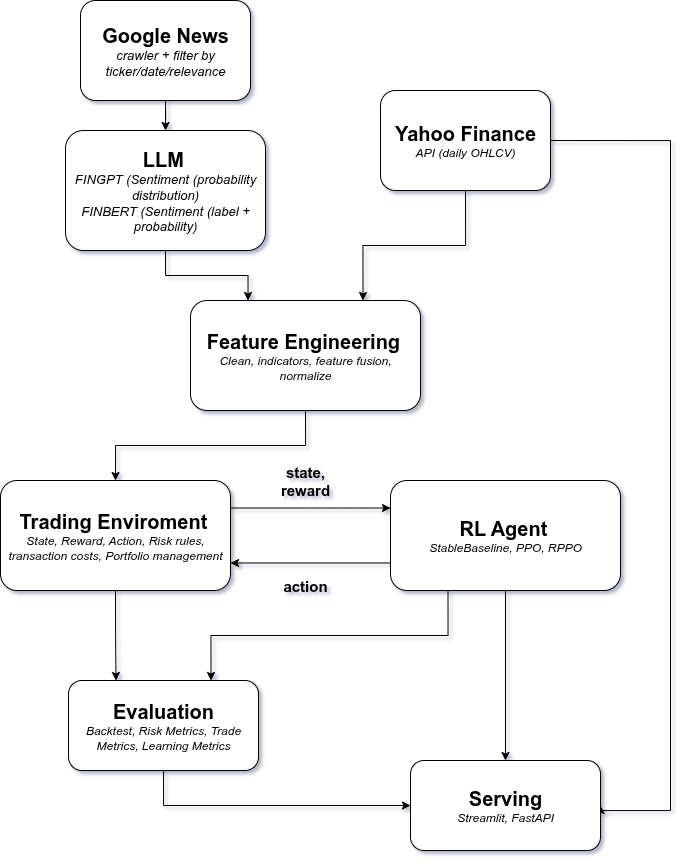
\includegraphics[width=\linewidth]{photos/finrlllm.drawio.png}
  \caption{Overall system architecture. Google News (crawler with ticker/date/relevance filters) and Yahoo Finance (API, daily OHLCV) feed into LLM sentiment (FinGPT: probability distribution; FinBERT: label+probability). Features are cleaned, normalized, and fused with technical indicators, forming the environment state (cash, holdings, OHLCV+sentiment+VIX). The PPO/RPPO agent outputs target allocations (softmax with per-asset cap), which are executed with transaction costs and turbulence risk rules. An evaluation module computes Sharpe, CAGR, and Max Drawdown on out-of-sample data. Results are served via Streamlit and FastAPI.}
  \label{fig:architecture}
\end{figure}


\paragraph{Component Interactions.}
\begin{enumerate}
    \item \textbf{Data ingestion.} Google News articles are collected via a custom crawler with ticker/date filters; Yahoo Finance provides daily OHLCV via an API. All items are timestamped in UTC and mapped to tickers.
    \item \textbf{LLM sentiment.} Each article/headline is routed to two models: \emph{FinGPT} outputs a probability distribution \(P(\text{pos},\text{neg},\text{neu})\); \emph{FinBERT} provides a hard label (pos/neg/neu) with its associated probability. These signals are aggregated per asset and aligned to trading bars (e.g., previous close).
    \item \textbf{Preprocessing \& feature fusion.} We de-duplicate, clean, and align records, compute technical indicators (EMA, MACD, RSI, ATR, Bollinger width, momentum/returns), normalize features, and fuse sentiment with OHLCV.
    \item \textbf{Environment.} The Gym-like environment exposes the fused state (cash, holdings, indicators, sentiment, VIX) and enforces action constraints (softmax weights with per-asset cap, no shorting), transaction costs (0.1\% buy/sell), and risk rules (turbulence soft/hard).
    \item \textbf{RL agent.} Using PPO and RPPO (Stable-Baselines3 contrib), the policy outputs logits mapped to target weights. The agent learns from rollouts generated by interacting with the environment.
    \item \textbf{Portfolio management.} Actions are converted to integer share orders, costs are applied, and the portfolio state (cash/holdings/P\&L) is updated.
    \item \textbf{Evaluation.} On a disjoint test set, the evaluator re-queries Yahoo Finance for prices, computes Sharpe, CAGR, and Max Drawdown, and compares against baselines (e.g., OHLCV-only, no-sentiment).
    \item \textbf{Serving.} Results and (optionally) live inference are exposed via a Streamlit dashboard and FastAPI endpoints.
\end{enumerate}

\paragraph{Design Rationale.}
Dual sentiment channels (FinGPT probabilities and FinBERT hard labels) provide complementary signals; their fusion with OHLCV and indicators enriches the state without leaking future information. Explicit turbulence controls and transaction costs keep the training dynamics realistic. The evaluation component re-fetches prices to ensure a clean separation between training and testing data sources. Finally, separating serving (Streamlit/FastAPI) from training enables reproducible offline experiments and modular deployment.

\section{Summary}

This chapter outlined the methodology and design of the proposed RL-based trading framework with LLM-driven sentiment integration. We first formalized the problem as an MDP with explicit state, action, reward, and risk-control definitions. We then described the system architecture, covering data ingestion, sentiment extraction, feature engineering, environment design, RL training, evaluation, and deployment. The design emphasizes realistic market constraints, reproducibility, and modularity. These methodological foundations provide the basis for the experimental setup and empirical analysis presented in the following chapter.


\chapter{Project Description}

\section{Introduction}

\section{Selected Market Description}

Initially, the cryptocurrency market was chosen as the target environment, with Bitcoin as the primary asset. I implemented basic reinforcement learning methods on this market and even incorporated sentiment analysis using large language models (LLMs). However, the results did not show meaningful improvements. Through further investigation, I realized that the cryptocurrency market is extremely volatile and highly complex, which made it difficult to achieve stable and consistent outcomes. Consequently, I decided to shift my focus to a different market.

After conducting additional research, I selected the U.S. stock market, specifically the Dow Jones Industrial Average (DOW30) index. To simplify the scope and reduce the complexity of working with a large number of stocks, I focused on a subset of four companies: Apple (AAPL), JPMorgan Chase (JPM), Boeing (BA), and Goldman Sachs (GS). This subset was deliberately chosen to include two stocks with abundant news coverage (AAPL and JPM) and two with comparatively limited news availability (BA and GS). 

Furthermore, the analysis in this project was conducted on a \textbf{daily basis}, rather than using higher-frequency data such as hourly or minute-level intervals. Daily data was chosen for several reasons:

\begin{enumerate}
    \item It is simpler to process and computationally less demanding.  
    \item It reduces the impact of short-term noise and extreme volatility.  
    \item It is more widely available and reliable compared to high-frequency data.  
    \item It aligns better with external information sources such as news and sentiment analysis, which are often reported daily.  
    \item It provides more stable and interpretable results for evaluating trading strategies.  
\end{enumerate}


The subsequent stages of this project were carried out using this subset of stocks as the primary environment.


\section{Data Collection}

The data required for this project can be divided into two main categories: (i) technical market data and (ii) news-related data.  

For the technical data, I collected standard financial indicators such as \textit{Open, Close, Low, High, and Volume (OCLHV)}, the \textit{Volatility Index (VIX)}, and the \textit{Turbulence Index}, among others. These datasets were obtained from \texttt{Yahoo Finance} using Python libraries, which provided a reliable, free, and well-documented source for financial market information.  

The more challenging part of data collection was gathering news-related data. Access to high-quality financial news sources often requires expensive subscriptions, and scraping such websites is usually restricted due to strict security and anti-bot measures. For the cryptocurrency market, I relied on \texttt{https://cryptoslate.com/}, which offered filtering options across different cryptocurrencies. Using this source, I was able to extract Bitcoin-related news covering a two-year period, from early 2024 to 2025. These extracted datasets have been made publicly available (link to be added).  

In contrast, the U.S. stock market presented an even greater challenge, as most reputable financial news outlets imposed stricter restrictions, making it difficult to obtain data in a systematic manner. To overcome this issue, I turned to \texttt{Google News}, which provides flexible query filters for ticker symbols, time ranges, and sorting options based on relevance and source credibility. Using this approach, I successfully collected news articles related to the four selected companies (AAPL, JPM, BA, GS) from 2010 to 2025.  

The extracted dataset includes the following fields: news headline, summary, link, publication date, \texttt{finbert\_label}, \texttt{finbert\_score}, \texttt{fingpt\_label}, and \texttt{fingpt\_score}. Details regarding the generation of these sentiment scores will be explained in the \textit{Sentiment Extraction from News} section.  

For the web scraping process, I used the Python \texttt{Selenium} library, which enabled automated browsing and data extraction from both CryptoSlate and Google News. The final processed datasets have been stored and shared (link to be added).

\section{Data Preprocessing}

Data preprocessing in this project was carried out in several stages.  

First, for the news data, since the initial output of the crawling process was in raw HTML format, it was necessary to parse and extract the relevant fields, such as headline, summary, publication date, and sentiment scores.  

Second, in order to build the final dataset, the extracted news articles needed to be merged with the corresponding technical market data on a daily basis. As there could be multiple news items published on the same day, an averaging method was applied to aggregate sentiment scores for that day.  

Moreover, considering that the impact of news may extend beyond the day of publication, a smoothing technique was applied. Specifically, an exponential moving average with a window size of 7 days and a decay factor of 0.8 was used. These hyperparameters were selected empirically. In practice, this means that the sentiment feature for a given day was influenced not only by the news of that day but also by the sentiment of the preceding week, with more recent news receiving higher weights.  

Finally, the input features were normalized before being fed into the model. Standard z-score normalization was applied to ensure that all features had zero mean and unit variance, which improves training stability and model performance.

\section{Data Analysis}

The primary analysis in this project focused on examining the relationship between sentiment scores and subsequent price changes over time. Specifically, I investigated whether the sentiment extracted from news articles could help predict future stock returns.

To this end, a Granger causality analysis based on a Vector Autoregression (VAR) model was employed. The Granger VAR test is a statistical method used to determine whether one time series can provide predictive information about another. In other words, if including past values of a sentiment score improves the prediction of stock returns compared to using only past returns, the sentiment series is said to ``Granger-cause'' the returns. This approach allows for testing the predictive power of multiple sentiment features simultaneously while accounting for lagged dependencies.

Before performing this analysis, it is necessary for all variables to be stationary, meaning their statistical properties (mean, variance) do not change over time. To achieve stationarity, the analysis was conducted on \textbf{returns} (calculated as the difference between consecutive closing prices) rather than raw prices. Similarly, sentiment scores from both FinBERT and FinGPT were aggregated on a daily basis and smoothed using a rolling mean with a window size of 7 days and a half-life of 2.5 days, reflecting the influence of news over several subsequent days.

The stationarity of each time series was formally tested using the Augmented Dickey-Fuller (ADF) test, which evaluates the null hypothesis that a unit root exists in the series (i.e., the series is non-stationary). If the null hypothesis is rejected, the series is considered stationary and suitable for VAR modeling.  

Using this approach, I was able to compare and evaluate the predictive performance of FinBERT and FinGPT sentiment scores in relation to daily stock returns. The detailed methodology for extracting these sentiment scores from news articles is described in the \textit{Sentiment Extraction from News} section. The results of the causality tests and predictive evaluations are presented and discussed in the \textit{Experiments and Results} chapter.

The following diagram illustrates the step-by-step procedure used in the analysis:

\begin{center}
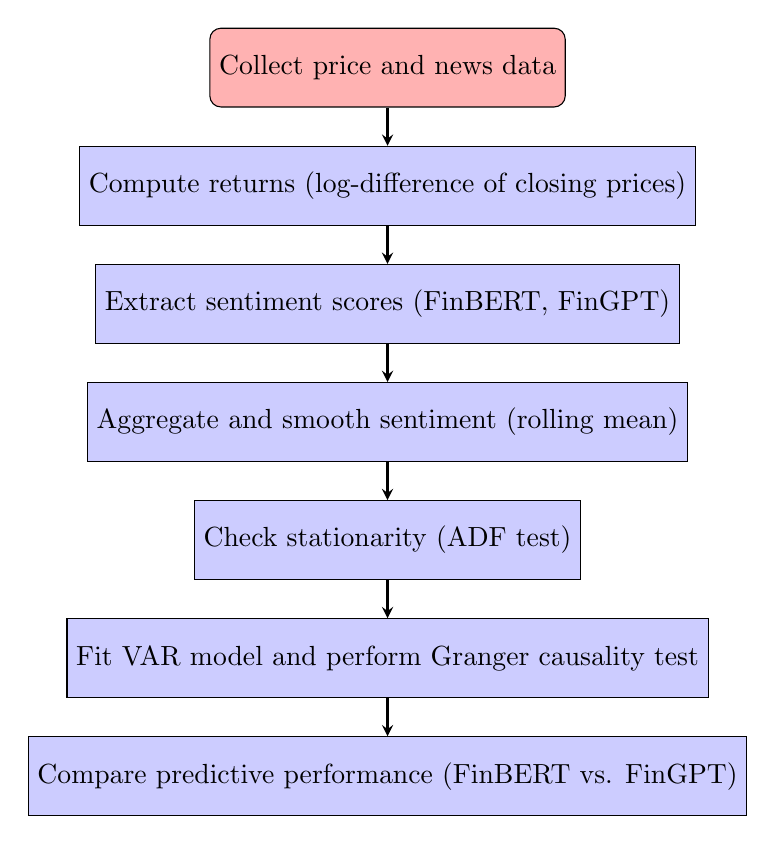
\begin{tikzpicture}[node distance=1.5cm]

\node (start) [startstop] {Collect price and news data};
\node (returns) [process, below of=start] {Compute returns (log-difference of closing prices)};
\node (sentiment) [process, below of=returns] {Extract sentiment scores (FinBERT, FinGPT)};
\node (smooth) [process, below of=sentiment] {Aggregate and smooth sentiment (rolling mean)};
\node (stationarity) [process, below of=smooth] {Check stationarity (ADF test)};
\node (var) [process, below of=stationarity] {Fit VAR model and perform Granger causality test};
\node (compare) [process, below of=var] {Compare predictive performance (FinBERT vs. FinGPT)};

\draw [arrow] (start) -- (returns);
\draw [arrow] (returns) -- (sentiment);
\draw [arrow] (sentiment) -- (smooth);
\draw [arrow] (smooth) -- (stationarity);
\draw [arrow] (stationarity) -- (var);
\draw [arrow] (var) -- (compare);

\end{tikzpicture}
\end{center}

\section{Sentiment Extraction from News}
\label{sec:sentiment_extraction}

This project employs two domain-specific language models for financial sentiment analysis: \textbf{FinBERT} and \textbf{FinGPT}. While both models output a probability distribution over \textit{positive}, \textit{negative}, and \textit{neutral}, they differ substantially in architecture, parameter count, training data, and inference complexity.

\subsection{FinBERT}
\label{subsec:finbert}
\textbf{FinBERT} is an encoder-only transformer derived from BERT-base and further adapted to the financial domain. It uses the standard BERT-base configuration (12 layers, 12 attention heads, hidden size 768; $\sim$110M parameters) and is domain-adapted by continued pretraining on large-scale financial text, then fine-tuned for sentiment classification on labeled datasets such as the Financial PhraseBank. In the publicly available \texttt{ProsusAI/finbert} checkpoint, the final classification head produces softmax probabilities over three labels: \textit{positive}, \textit{negative}, and \textit{neutral} \cite{araci2019finbert}.

\subsection{FinGPT (Llama~3 + LoRA adapters)}
\label{subsec:fingpt}
\textbf{FinGPT} is a decoder-only large language model based on the \texttt{meta-llama/Meta-Llama-3-8B} backbone, adapted to finance via low-rank adapters (LoRA) and instruction-style fine-tuning. The released checkpoint \texttt{FinGPT/fingpt-mt\_llama3-8b\_lora} attaches lightweight LoRA modules to the frozen base model, enabling domain-specific adaptation with only a small fraction of trainable parameters. The FinGPT initiative follows a data-centric pipeline: automatic curation of financial data (e.g., news, filings, social media, QA pairs) and lightweight adaptation of open-weight LLMs. For sentiment analysis, FinGPT is trained to follow instructions and generate one of \textit{positive}, \textit{negative}, or \textit{neutral} labels \cite{yang2023fingpt}.

\subsection{Numerical Sentiment Scoring}
For both models, the raw output is a probability distribution across the three sentiment classes. To convert this distribution into a single numerical score, I adopted a simple yet effective approach: the difference between the predicted probabilities of the \textit{positive} and \textit{negative} classes. Formally,
\[
\text{Sentiment Score} = P(\text{positive}) - P(\text{negative}).
\]
This formulation ensures that higher scores correspond to more positive sentiment, lower scores correspond to more negative sentiment, and values near zero indicate neutrality.


\section{Trading Environment}
\label{sec:rl_env}

This part of the project consists of two main components: the \textbf{trading environment} and the \textbf{reinforcement learning (RL) agent}. The environment simulates market dynamics and risk conditions, while the RL agent learns trading strategies through repeated interaction.

\subsection{Customized Trading Environment}
As the starting point, I adopted the open-source environment provided in the FinRL library\footnote{\url{https://github.com/AI4Finance-Foundation/FinRL/blob/master/finrl/meta/env_stock_trading/env_stocktrading.py}}. Due to its open-source nature, the environment was extensively customized. The main modifications include:
\begin{itemize}
    \item A redesigned \textbf{state space} with additional technical, sentiment, and risk features.
    \item Redefinition of the \textbf{reward function} to better reflect portfolio performance.
    \item A turbulence-based \textbf{risk control mechanism}.
    \item Support for \textbf{multi-environment training} to improve robustness.
    \item \textbf{Episode randomization} with variable start dates and lengths.
    \item A new \textbf{action execution mechanism} based on portfolio weights.
\end{itemize}

\subsection{State Space}
The final state representation integrates technical indicators, risk measures, sentiment signals, and portfolio information. Each feature is normalized to ensure comparability across stocks. Technical indicators were computed using the open-source \texttt{ta} library\footnote{\url{https://github.com/bukosabino/ta}}, which provides efficient implementations of standard market indicators. The full set of features includes:


\begin{itemize}
    \item \textbf{20-day momentum (mom\_20d):} relative price change over the past 20 days, capturing short-term momentum.
    \item \textbf{Exponential moving averages (ema\_20, ema\_60):} short- and medium-term price trends.
    \item \textbf{MACD and signal line:} momentum indicators used to detect trend changes.
    \item \textbf{Relative Strength Index (RSI, 14-day):} oscillator detecting overbought or oversold conditions.
    \item \textbf{Average True Range (ATR, 14-day):} measure of market volatility based on trading ranges.
    \item \textbf{Bollinger Band Width:} volatility measure derived from the spread of Bollinger Bands.
    \item \textbf{Normalized closing price (zclose\_60):} price scaled relative to a 60-day rolling window.
    \item \textbf{Daily return (ret\_1d):} one-day return capturing immediate asset performance.
    \item \textbf{Sentiment scores (finbert\_future, fingpt\_future):} NLP-based market sentiment extracted from financial news using FinBERT and FinGPT.
    \item \textbf{On-Balance Volume (OBV):} volume-based indicator reflecting the flow of capital.
    \item \textbf{Normalized VIX:} index of market-wide volatility, representing systemic risk.
    \item \textbf{Portfolio state:} normalized number of shares per stock and normalized cash balance.
\end{itemize}

\subsection{Reward Function}
Two reward definitions were evaluated:
\begin{enumerate}
    \item \textbf{Portfolio log return:}
    \[
    R_t = \frac{A_{t+1} - A_t}{A_t + 10^{-8}} \cdot \frac{n_{\text{days}}}{T} \cdot \text{scale},
    \]
    where $A_t$ is portfolio value at time $t$, $T$ is episode length, and \textit{scale} is a normalization constant.
    \item \textbf{Alternative metric:} [\textit{Placeholder – to be detailed in final version.}]
\end{enumerate}

\subsection{Risk Control via Turbulence}
To manage exposure during volatile periods, a turbulence-based mechanism was implemented. Turbulence quantifies abnormal market conditions by comparing price movements against historical covariance. Two thresholds were applied:
\begin{itemize}
    \item \textbf{Soft threshold} ($\tau_{soft} = 70$): when exceeded, no new buy orders are executed.
    \item \textbf{Hard threshold} ($\tau_{hard} = 100$): when exceeded, all current positions are liquidated and no further purchases are allowed.
\end{itemize}

This mechanism enforces defensive behavior under stress conditions.

\subsection{Episode Randomization}
The default FinRL environment defines episodes as fixed intervals starting from the first trading day and ending at the last day of the dataset. While this provides a consistent training setup, it reduces the variability of market conditions experienced by the agent. To address this limitation, I introduced \textbf{episode randomization}.

Formally, let $T$ denote the total number of trading days in the dataset and $L_{\min}$ the minimum allowed episode length. At the beginning of each episode, a random starting day $s$ is sampled such that
\[
s \sim \text{Uniform}(0, T - L_{\min}).
\]
The corresponding episode length $L$ is then sampled from the interval
\[
L \sim \text{Uniform}(L_{\min}, T - s).
\]
The episode runs from $s$ to $s + L$, ensuring that the minimum duration constraint is satisfied. With a small probability, the full dataset is used ($s=0$, $L=T$) to maintain consistency with the original setup.

This randomization strategy exposes the agent to diverse subperiods of the market, improving generalization by:
\begin{itemize}
    \item Preventing overfitting to specific temporal patterns.
    \item Simulating training conditions closer to real-world online trading, where entry dates and horizons vary.
    \item Increasing robustness to different volatility regimes and market cycles.
\end{itemize}

\subsection{Action Execution Mechanism}
In the default FinRL implementation, the action for each stock $i$ is a scalar $a_i \in [-1,1]$ that is multiplied by a constant $h_{\max}$ to determine the number of shares to buy or sell. This formulation suffers from several issues:
\begin{itemize}
    \item It does not scale with the total portfolio value $A_t$.
    \item It ignores differences in stock prices $p_{i,t}$.
    \item It restricts the agent to fixed trading sizes regardless of market conditions.
\end{itemize}

To overcome these limitations, I reformulated the action as a \textbf{portfolio allocation problem}. Let $\mathbf{z} \in \mathbb{R}^N$ denote the raw action logits for $N$ assets (plus one dummy cash component). The logits are mapped to normalized portfolio weights $\mathbf{w}$ using the softmax transformation:
\[
w_i = \frac{\exp(z_i)}{\sum_{j=1}^{N+1} \exp(z_j)}, \quad i=1,\dots,N+1,
\]
with $\sum_{i=1}^{N+1} w_i = 1$.

A maximum allocation cap is applied to prevent over-concentration in any single asset:
\[
w_i^{\text{capped}} = \min(w_i, \, c), \quad c=0.5.
\]

The target dollar allocation for stock $i$ is then given by
\[
d_{i,t} = w_i^{\text{capped}} \cdot A_t,
\]
where $A_t$ is the current portfolio value. The target number of shares is
\[
q_{i,t}^{\text{target}} = \left\lfloor \frac{d_{i,t}}{p_{i,t}} \right\rfloor,
\]
where $p_{i,t}$ is the stock’s price at time $t$. The required trade volume is
\[
\Delta q_{i,t} = q_{i,t}^{\text{target}} - q_{i,t}^{\text{current}}.
\]

The turbulence thresholds (Section~\ref{sec:rl_env}) are then applied:
\begin{itemize}
    \item If turbulence $> \tau_{\text{hard}}$, all $q_{i,t}$ are set to zero (forced liquidation).
    \item If $\tau_{\text{soft}} < \text{turbulence} \leq \tau_{\text{hard}}$, no buy orders are executed, i.e., $\Delta q_{i,t} = \min(0, \Delta q_{i,t})$.
\end{itemize}

This formulation has several advantages:
\begin{itemize}
    \item Actions scale with portfolio value and stock prices.
    \item The agent effectively learns an allocation strategy rather than arbitrary share counts.
    \item Risk is explicitly controlled through allocation caps and turbulence overrides.
\end{itemize}

\subsection{Summary}
The customized environment provides:
\begin{itemize}
    \item A comprehensive and informative state representation.
    \item Reward functions linked directly to portfolio performance.
    \item Explicit turbulence-based risk management.
    \item Greater training diversity via randomized episodes.
    \item A robust action mechanism based on portfolio weights.
\end{itemize}

For implementation, the \texttt{Gymnasium} library was used, which enables seamless integration with most reinforcement learning agents and frameworks.  


\section{RL Agent}
\label{sec:rl_agent}

To implement the reinforcement learning agent, the \texttt{Stable-Baselines3 (SB3)} library\footnote{\url{https://github.com/DLR-RM/stable-baselines3}} and its extension \texttt{sb3-contrib} were employed. These libraries provide reliable implementations of modern RL algorithms and support seamless interaction with the \texttt{Gymnasium} framework, ensuring full compatibility with the customized trading environment.

\subsection{Implementation Framework}
A dedicated agent wrapper was designed to streamline experimentation with different algorithms. The implementation provides the following core functionalities:
\begin{itemize}
    \item \textbf{Model initialization:} loading RL models with default or customized hyperparameters.
    \item \textbf{Training:} executing training processes with integrated logging and callback mechanisms.
    \item \textbf{Prediction:} running inference on unseen market data while recording portfolio evolution and executed actions.
\end{itemize}

\subsection{Evaluated Algorithms}
Several reinforcement learning algorithms from SB3 and \texttt{sb3-contrib} were evaluated on the validation dataset, including:
\begin{itemize}
    \item \texttt{A2C}, \texttt{PPO}, \texttt{SAC}, \texttt{TD3} (from SB3),
    \item \texttt{RecurrentPPO}, \texttt{CrossQ}, \texttt{TRPO} (from sb3-contrib).
\end{itemize}

Among these, two algorithms were selected for final experiments based on validation performance: \textbf{Proximal Policy Optimization (PPO)} and \textbf{Recurrent Proximal Policy Optimization (RecurrentPPO)}.

\paragraph{PPO.}
PPO is a policy-gradient method that stabilizes training by constraining policy updates through a clipped surrogate objective. This prevents excessively large updates, ensuring balanced exploration and exploitation. PPO has become one of the most widely used RL algorithms in continuous control problems such as financial trading, thanks to its robustness and simplicity.

\paragraph{RecurrentPPO.}
RecurrentPPO extends the PPO framework by incorporating recurrent neural networks (e.g., LSTM) into the policy architecture. This enhancement allows the agent to capture temporal dependencies and retain information about past states, which is highly beneficial in financial markets where historical context and time-series patterns influence decision-making.

\subsection{Hyperparameter Optimization}
The performance of reinforcement learning algorithms is highly sensitive to hyperparameter choices such as learning rate, discount factor, batch size, and clipping range. To systematically tune these parameters, the \texttt{Optuna} library\footnote{\url{https://optuna.org/}} was employed. Hyperparameter search was performed on the validation dataset to achieve robust configurations while avoiding overfitting.

The optimized hyperparameters and their corresponding results are reported in Chapter \textit{Experiments and Results}.

\section{Monitoring}
\label{sec:monitoring}

Monitoring is a crucial component in the training and evaluation of reinforcement learning models, especially in financial domains where performance is highly sensitive to hyperparameters and market regimes. To address this, an improved monitoring framework was implemented, extending the basic functionality provided in the FinRL library.

\subsection{Approach}
Training progress was tracked using callback mechanisms that log key signals such as rewards, episode lengths, and learning rates. These were integrated with visualization tools including \texttt{TensorBoard} and \texttt{Weights \& Biases (W\&B)}, enabling real-time inspection of learning dynamics. Compared to the default setup, the monitoring framework was enhanced to provide more reliable insights into model behavior during training.

\subsection{Benefits}
This monitoring setup made it possible to:
\begin{itemize}
    \item Detect instabilities or divergence early in the training process.
    \item Compare different algorithms and hyperparameter configurations systematically.
    \item Evaluate model performance across different training and validation phases with greater clarity.
\end{itemize}

\subsection{Summary}
Overall, the improved monitoring framework played a central role in guiding model development. By continuously tracking learning curves and performance metrics, it facilitated effective hyperparameter tuning and robust evaluation of reinforcement learning agents.


\section{Serving and Deployment}
\label{sec:deployment}

To enable practical use of the trained reinforcement learning models, a serving and deployment pipeline was developed. The system consists of two main components: a \textbf{backend service} implemented with \texttt{FastAPI}, and a \textbf{frontend interface} built using \texttt{Streamlit}.

\subsection{Backend}
The backend is responsible for loading trained models and providing a set of APIs to interact with them. Its main functionalities include:
\begin{itemize}
    \item Managing model inference by receiving requests and returning predicted actions.
    \item Handling portfolio-related operations, such as retrieving open and closed positions.
    \item Preparing data pipelines to ensure consistency between incoming requests and the model’s expected input format.
\end{itemize}

\subsection{Frontend}
The frontend provides a user-friendly interface for visualization and interaction. It consists of three main sections:
\begin{enumerate}
    \item \textbf{Price charts:} visualization of the closing price of each stock over a user-specified time horizon.
    \item \textbf{Technical analysis:} computation and display of selected technical indicators and features within the chosen period.
    \item \textbf{Trading actions:} selection of a time interval to extract the agent’s actions and display corresponding open and closed positions for each stock.
\end{enumerate}

\subsection{Summary}
This deployment framework enables end-to-end interaction with the RL trading agent. The backend ensures efficient model serving, while the frontend provides intuitive visualization and analysis tools for users to explore market data, technical indicators, and model-driven trading decisions.

\section{Summary}

\chapter{Implementation}

\section{Introduction}

\section{Tools and Frameworks}

The project was implemented in \textbf{Python 3}, which provides a rich ecosystem for data science, reinforcement learning, and deployment. 
Table~\ref{tab:tools_frameworks} summarizes the main tools and libraries used, grouped by functionality.
\begin{table}[H]
\centering
\renewcommand{\arraystretch}{1.3} % more row spacing
\begin{tabular}{p{4cm} p{10cm}}
\hline
\textbf{Category} & \textbf{Tools and Purpose} \\
\hline

\textbf{Data Acquisition} 
 & \texttt{yfinance} -- retrieve OHLCV market data (Yahoo Finance API). \\
 & \texttt{Selenium} -- crawl Google News articles with ticker/date/relevance filters. \\[0.5em]

\textbf{Data Processing \& Features} 
 & \texttt{pandas}, \texttt{numpy} -- data wrangling, preprocessing, normalization. \\
 & \texttt{ta} -- computation of technical indicators (EMA, MACD, RSI, ATR, Bollinger). \\
 & \texttt{json} -- configuration and results storage. \\[0.5em]

\textbf{Environment} 
 & \texttt{gymnasium} -- base RL environment API. \\
 & \texttt{FinRL} -- prototyping and customization of trading environments. \\[0.5em]

\textbf{Reinforcement Learning} 
 & \texttt{stable\_baselines3} -- implementations of PPO, A2C, DQN. \\
 & \texttt{sb3-contrib} -- RPPO extension. \\
 & \texttt{torch} -- underlying deep learning engine for model training and checkpointing. \\[0.5em]

\textbf{Hyperparameter Optimization} 
 & \texttt{Optuna} -- automated tuning of hyperparameters on validation data. \\[0.5em]

\textbf{Experiment Tracking} 
 & \texttt{wandb} (Weights \& Biases) -- experiment logging, visualization, and comparison. \\[0.5em]

\textbf{Evaluation and Benchmarking} 
 & \texttt{scipy} -- numerical evaluation utilities. \\
 & \texttt{PyPortfolioOpt (pypfopt)} -- mean-variance optimization baseline. \\[0.5em]

\textbf{Visualization} 
 & \texttt{matplotlib}, \texttt{seaborn} -- static performance plots. \\
 & \texttt{plotly} -- interactive equity curves and portfolio allocation plots. \\[0.5em]

\textbf{Deployment and Serving} 
 & \texttt{Streamlit} -- dashboard interface. \\
 & \texttt{FastAPI} -- REST API for model serving. \\
 & \texttt{requests} -- API communication. \\
 & \texttt{gdown} -- exchange of models/data with Google Drive. \\[0.5em]

\textbf{Utility} 
 & Python \texttt{logging} -- experiment logging and reproducibility. \\

\hline
\end{tabular}
\caption{Summary of tools and frameworks used in implementation.}
\label{tab:tools_frameworks}
\end{table}


Overall, this stack enabled rapid prototyping (FinRL), robust RL training (Stable-Baselines3 with PyTorch), automated data ingestion (yfinance, Selenium), reproducible experiment tracking (wandb), and deployment (Streamlit, FastAPI).

\section{Reproducibility and Environment}

Experiments were conducted in Python with PyTorch and Stable-Baselines3. 
The environment was GPU-enabled.  

Random seeds were not explicitly fixed across all frameworks. 
As a result, individual runs can differ slightly due to stochastic elements in reinforcement learning 
(e.g., policy initialization, exploration, and GPU nondeterminism). 
To mitigate this, each experiment was repeated multiple times, and average results across ten runs are reported 
in Chapter~6 to ensure robustness. 

Data reproducibility was ensured by recording snapshot dates for Yahoo Finance data 
and timestamping all Google News crawls. 
All times were normalized to UTC, and feature engineering strictly avoided look-ahead bias.


\section{Hardware and Computational Resources}

Experiments were conducted using a combination of cloud resources for training and inference, 
supplemented by a local laptop for deployment and lightweight testing. 

\paragraph{Kaggle (Training).} 
Most reinforcement learning training was carried out on the Kaggle Notebook environment 
with an \textbf{NVIDIA Tesla P100 GPU (16 GB VRAM)}, 
up to \textbf{13 GB RAM}, and \textbf{73 GB disk space}. 
Disk storage on Kaggle is only persistent through Datasets/Notebooks, 
so model checkpoints and logs were exported externally after each run. 

\paragraph{Google Colab Pro (LLM Inference).} 
Colab Pro was used specifically for natural language processing tasks, 
namely inference with large language models (\textbf{FinGPT} and \textbf{FinBERT}) 
to extract sentiment from Google News articles. 
This required access to a \textbf{high-memory runtime (up to 52 GB RAM)} 
and an \textbf{NVIDIA A100 GPU (40 GB VRAM)} for faster batch inference. 
Training of RL agents was not performed on Colab Pro. 

\paragraph{Local Laptop (Deployment).} 
For deployment and testing of the final system, a personal laptop running 
\textbf{Ubuntu 22.04}, equipped with an \textbf{Intel CPU}, 
\textbf{16 GB RAM}, and an entry-level \textbf{NVIDIA MX140 GPU (2 GB VRAM)}, 
was used. This setup was sufficient for running the trained models via FastAPI and 
visualizing results through Streamlit, though not powerful enough for large-scale training. 

\paragraph{Compute Configuration.} 
Across training experiments, we used 1--4 parallel environments in Stable-Baselines3, 
batch sizes between 256 and 1024, and total timesteps between 400k and 1.5M depending on the algorithm. 
Each experiment was repeated independently 3--10 times to account for stochasticity. 
Training time per run ranged from approximately 30 minutes to 3 hours, 
depending on the GPU, algorithm, and configuration.

\section{Summary}



\chapter{Experiments and Results}


\section{Stationarity Analysis: Closing Prices vs.\ Returns}

\subsection{Methodology}
To examine whether price levels or returns should be used in modeling, we applied the
Augmented Dickey--Fuller (ADF) unit root test \cite{dickey1979distribution}. The null
hypothesis $H_0$ is that the series possesses a unit root (i.e., is non-stationary).  
We conducted the test on daily adjusted closing prices and their log-returns for
four Dow Jones constituents (AAPL, BA, GS, JPM) over the period
2010-01-01 to 2025-09-07.  
The tests used automatic lag length selection via AIC.

\subsection{Results}
Table~\ref{tab:adf-results} summarizes the ADF test outcomes. For all four stocks,
the closing price series exhibit large p-values ($>0.05$), meaning we cannot reject
the null hypothesis of a unit root. This indicates that price levels are non-stationary.
In contrast, the log-return series show strongly negative test statistics with
extremely small p-values ($<0.01$), allowing us to reject the null and conclude that
returns are stationary.

\begin{table}[H]
\centering
\caption{ADF test results for closing prices and log-returns (2010--2025).}
\label{tab:adf-results}
\begin{tabular}{lrrrrr}
\toprule
\textbf{Stock} & \textbf{Series} & \textbf{ADF Stat.} & \textbf{p-value} & \textbf{Lags} & \textbf{Decision (5\%)} \\
\midrule
AAPL & Close Price  &  0.735  & 0.991 & 33 & Non-stationary \\
AAPL & Log Return   & -16.602 & 0.000 & 19 & Stationary \\
\midrule
BA   & Close Price  & -1.818  & 0.371 & 34 & Non-stationary \\
BA   & Log Return   & -12.967 & 0.000 & 34 & Stationary \\
\midrule
GS   & Close Price  &  1.895  & 0.999 & 31 & Non-stationary \\
GS   & Log Return   & -24.675 & 0.000 &  8 & Stationary \\
\midrule
JPM  & Close Price  &  2.377  & 0.999 & 29 & Non-stationary \\
JPM  & Log Return   & -17.571 & 0.000 & 20 & Stationary \\
\bottomrule
\end{tabular}
\end{table}

\subsection{Discussion}
The findings align with established financial econometrics: asset price levels typically
follow a stochastic trend and are non-stationary, while log-returns are stationary.
This result justifies the use of returns rather than prices in reinforcement learning
state representations and reward computations. When price levels are required (e.g.,
for portfolio value scaling), appropriate transformations such as differencing or
normalization are applied to mitigate non-stationarity.



\section{Causality Analysis: Sentiment Models and Market Returns}

\subsection{Methodology}
To assess whether sentiment information helps explain market dynamics, we conducted
Granger causality analysis using a Vector Autoregression (VAR) framework
\cite{granger1969investigating}. For each stock (AAPL, BA, GS, JPM), we considered
daily log-returns as the dependent variable and included exponentially smoothed
FinBERT and FinGPT sentiment scores (7-day EWMA, half-life 2.5) as predictors.
The optimal lag length was selected by information criteria (AIC, BIC, HQIC, FPE),
with a maximum of 10 lags.  
We then tested (i) whether FinBERT or FinGPT individually Granger-cause returns,
and (ii) whether they jointly Granger-cause returns.

\subsection{Results}
Table~\ref{tab:granger} reports the F-statistics and p-values. The evidence is mixed
across stocks:
\begin{itemize}
    \item For \textbf{AAPL}, FinGPT shows significant predictive power ($p=0.021$),
    while FinBERT alone does not. The joint test strongly rejects the null
    ($p<0.001$), suggesting that sentiment features combined improve return prediction.
    \item For \textbf{BA}, neither FinBERT nor FinGPT individually exhibits
    significant causality, and the joint test is not significant ($p=0.333$).
    \item For \textbf{GS}, none of the predictors show significance; all p-values
    exceed 0.19.
    \item For \textbf{JPM}, both predictors are marginally significant
    ($p\approx0.07$--$0.08$), and the joint test is significant at the 5\% level
    ($p=0.028$).
\end{itemize}

\begin{table}[H]
\centering
\caption{Granger causality tests of FinBERT and FinGPT sentiment on stock returns.}
\label{tab:granger}
\begin{tabular}{l l r r}
\toprule
\textbf{Stock} & \textbf{Predictor} & \textbf{F-stat} & \textbf{p-value} \\
\midrule
AAPL & FinBERT & 1.387 & 0.197 \\
     & FinGPT  & 2.259 & 0.021 \\
     & Joint   & 2.812 & $<0.001$ \\
\midrule
BA   & FinBERT & 0.865 & 0.565 \\
     & FinGPT  & 1.791 & 0.057 \\
     & Joint   & 1.107 & 0.333 \\
\midrule
GS   & FinBERT & 1.307 & 0.227 \\
     & FinGPT  & 0.668 & 0.739 \\
     & Joint   & 1.271 & 0.196 \\
\midrule
JPM  & FinBERT & 1.754 & 0.072 \\
     & FinGPT  & 1.723 & 0.078 \\
     & Joint   & 1.728 & 0.028 \\
\bottomrule
\end{tabular}
\end{table}

\subsection{Discussion}
Overall, the results indicate that sentiment signals have heterogeneous predictive
power across stocks. FinGPT exhibits stronger evidence of causality compared to FinBERT,
especially for AAPL and JPM. While individual causality is often weak, joint tests
reveal that combining both sentiment measures can significantly improve explanatory
power for certain tickers. This suggests that reinforcement learning agents may benefit
from incorporating multiple sentiment sources rather than relying on a single model.


\section{Trading Agent Evaluation: Algorithms, Environments, and Setups}

\subsection{Overview of Experimental Dimensions}

\paragraph{PPO vs.\ RPPO}
Proximal Policy Optimization (PPO) serves as the baseline on-policy algorithm, while 
Regularized PPO (RPPO) extends it with additional regularization terms to improve stability 
and generalization.

\paragraph{Raw Normalized Return vs.\ Log-Risk Adjusted Reward}
The Raw Normalized Return reward is proportional to portfolio-level normalized returns, 
while the Log-Risk Adjusted reward uses the logarithm of one-step returns to penalize 
large negative outcomes and emphasize risk sensitivity.

\paragraph{Single vs.\ Vectorized Environments}
Single-environment setups train the agent on one market trajectory per update, 
whereas the vectorized setup (3-env) runs three environments in parallel to 
increase sample efficiency and exposure to diverse scenarios.

\paragraph{Normal vs.\ Randomized Episodes}
Normal episodes follow fixed start and length windows, 
while randomized episodes sample variable start dates and episode lengths 
(minimum 1500 steps), increasing training diversity.

\vspace{0.75cm}

Before presenting the outcomes, it is important to note that each configuration was 
executed multiple times (10--15 independent runs) to account for stochasticity in 
reinforcement learning training. Reported values are averaged across runs to ensure 
robustness of the comparisons. 

The backtests were conducted over the period from \texttt{2023-01-03} to 
\texttt{2025-08-29}. 

In the following, we examine the results across the different setups, organized by 
algorithm, reward formulation, environment type, and episode structure.


\subsection{PPO}

\subsubsection{Raw Normalized Return Reward}

\paragraph{Single Environment}

\subparagraph{Normal Episodes}

\Needspace{12\baselineskip} % ensure space; otherwise start a new page
\begin{center}
\begin{tabular}{l c}
\toprule
\textbf{Metric} & \textbf{Mean $\pm$ Std} \\
\midrule
Annualized Return [\%]      & 25.65 $\pm$ 4.47 \\
Annualized Volatility [\%]  & 20.46 $\pm$ 1.07 \\
Max Drawdown [\%]           & -24.78 $\pm$ 1.82 \\
Average Drawdown [\%]       & -5.33 $\pm$ 0.57 \\
Sharpe Ratio                & 1.22 $\pm$ 0.19 \\
Sortino Ratio               & 1.58 $\pm$ 0.24 \\
Calmar Ratio                & 1.04 $\pm$ 0.19 \\
Number of Trades            & 122.50 $\pm$ 58.41 \\
\bottomrule
\end{tabular}
\captionof{table}{PPO -- Raw Normalized Return Reward -- Single Environment -- Normal Episodes}
\label{tab:ppo-raw-1env-normal}
\end{center}

\subparagraph{Randomized Episodes}

\Needspace{12\baselineskip} % ensure space; otherwise start a new page
\begin{center}
\begin{tabular}{l c}
\toprule
\textbf{Metric} & \textbf{Mean $\pm$ Std} \\
\midrule
Annualized Return [\%]: 21.35 $\pm$ 4.97 \\
Annualized Volatility [\%]: 19.25 $\pm$ 2.13 \\
Max Drawdown [\%]: -23.43 $\pm$ 1.94 \\
Average Drawdown [\%]: -6.05 $\pm$ 1.58 \\
Sharpe Ratio: 1.11 $\pm$ 0.22 \\
Sortino Ratio: 1.48 $\pm$ 0.29 \\
Calmar Ratio: 0.91 $\pm$ 0.20 \\
Number of Trades: 124.70 $\pm$ 47.89 \\
\bottomrule
\end{tabular}
\captionof{table}{PPO -- Raw Normalized Return Reward -- Single Environment -- Randomized Episodes}
\label{tab:ppo-raw-1env-random}
\end{center}

\paragraph{Vectorized Environments (3-env)}
\subparagraph{Normal Episodes}

\Needspace{12\baselineskip} % ensure space; otherwise start a new page
\begin{center}
\begin{tabular}{l c}
\toprule
\textbf{Metric} & \textbf{Mean $\pm$ Std} \\
\midrule
Annualized Return [\%]      & 20.78 $\pm$ 1.51 \\
Annualized Volatility [\%]  & 21.65 $\pm$ 1.17 \\
Max Drawdown [\%]           & -24.29 $\pm$ 2.54 \\
Average Drawdown [\%]       & -7.38 $\pm$ 0.89 \\
Sharpe Ratio                & 0.98 $\pm$ 0.06 \\
Sortino Ratio               & 1.32 $\pm$ 0.07 \\
Calmar Ratio                & 0.86 $\pm$ 0.11 \\
Number of Trades            & 144.50 $\pm$ 5.32 \\
\bottomrule
\end{tabular}
\captionof{table}{PPO -- Raw Normalized Return Reward -- Vectorized Environments (3-env) -- Normal Episodes}
\label{tab:ppo-raw-3env-normal}
\end{center}

\subparagraph{Randomized Episodes}

\Needspace{12\baselineskip} % ensure space; otherwise start a new page
\begin{center}
\begin{tabular}{l c}
\toprule
\textbf{Metric} & \textbf{Mean $\pm$ Std} \\
\midrule
Annualized Return [\%]      & 19.50 $\pm$ 1.05 \\
Annualized Volatility [\%]  & 19.28 $\pm$ 3.71 \\
Max Drawdown [\%]           & -23.89 $\pm$ 2.48 \\
Average Drawdown [\%]       & -6.14 $\pm$ 2.34 \\
Sharpe Ratio                & 1.04 $\pm$ 0.21 \\
Sortino Ratio               & 1.43 $\pm$ 0.29 \\
Calmar Ratio                & 0.82 $\pm$ 0.13 \\
Number of Trades            & 147.50 $\pm$ 2.12 \\
\bottomrule
\end{tabular}
\captionof{table}{PPO -- Raw Normalized Return Reward -- Vectorized Environments (3-env) -- Randomized Episodes}
\label{tab:ppo-raw-3env-random}
\end{center}

\subsubsection{Log-Risk Adjusted Reward}
\paragraph{Single Environment}
% description + results
\paragraph{Vectorized Environments (3-env)}
% description + results

\subsection{RPPO}
\subsubsection{Raw Normalized Return Reward}
\paragraph{Single Environment}
\subparagraph{Normal Episodes}
% description + results
\subparagraph{Randomized Episodes}
% description + results

\paragraph{Vectorized Environments (3-env)}
\subparagraph{Normal Episodes}
% description + results
\subparagraph{Randomized Episodes}
% description + results

\subsubsection{Log-Risk Adjusted Reward}
\paragraph{Single Environment}
% description + results
\paragraph{Vectorized Environments (3-env)}
% description + results


\section{Summary}


\chapter{Discussion and Analysis}

\section{Introduction}

\section{Summary}

\chapter{Conclusion and Future Work}

% -----------------------------
% References
% -----------------------------
\bibliographystyle{ieeetr}
\bibliography{references} % your .bib file

% -----------------------------
% Appendices (Lettered)
% -----------------------------
\appendix

\chapter{Appendix A: Title of Appendix}
% Content for Appendix A

\chapter{Appendix B: Title of Appendix}
% Content for Appendix B

\end{document}
